\renewcommand\chapterillustration{abertura-cartografia.jpg}
\renewcommand\chapterwhat{Projeções cartográficas. Classificação das projeções cartográficas quanto à superfície de projeção (planas, cônicas e cilíndricas) e quanto as propriedades (equivalentes, equidistantes, conformes e afiláticas).}
\renewcommand\chapterbecause{Projeções cartográficas são projeções da superfície terrestre no plano que possibilitam a visualização de uma área muito grande em uma única folha. Tornando possível, por exemplo, o planejamento de rotas ou organizações territoriais de um país inteiro em cima de uma mesa. Existem diferentes tipos de projeções e cada uma possui algum tipo de distorção (em relação a área, ângulo ou distância). As projeções cartográficas mais conhecidas são as cônicas, planas e cilíndricas, portanto serão a essas que daremos ênfase no capítulo.}
\chapter{Projeções Cartográficas}



\mbox{}\thispagestyle{empty}\clearpage

\thispagestyle{empty}

\begin{center}
Projeto: LIVRO ABERTO DE MATEMÁTICA

\noindent \begin{tabular}{lcccr}

\includegraphics[scale=.15]{impa}& \quad\quad& 
\includegraphics[width=3cm]{logo} & \quad\quad& 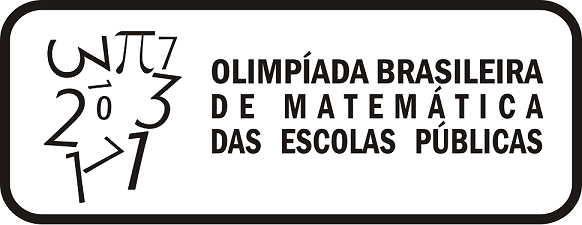
\includegraphics[scale=.24]{obmep} 
\end{tabular}
\end{center}

\vspace*{.3cm}

Cadastre-se como colaborador no site do projeto: \url{umlivroaberto.com}

Versão digital do capítulo:

\url{https://www.umlivroaberto.org/BookCloud/Volume_1/master/view/AF107.html}


\begin{tabular}{p{.15\textwidth}p{.7\textwidth}}
Título: & Projeções Cartográficas\\
\\
Ano/ Versão: & 2020 / versão 0.2 de 15 de agosto de 2020\\
\\
Editora & Instituto Nacional de Matem\'atica Pura e Aplicada (IMPA-OS)\\
\\
Realização:& Olimp\'iada Brasileira de Matem\'atica das Escolas P\'ublicas (OBMEP)\\
\\
Produção:& Livro Aberto\\
\\
Coordenação:& Fabio Simas e Augusto Teixeira (livroaberto@impa.br)\\
\\
  Autores: & Carmen Vieira Mathias (UFSM)\\
             & Lucas Schimith Zanon (SEDUC - RS)\\
\\
Revisoras: &  Lhaylla Crissaf (UFF) \\
\\
Design: & Andreza Moreira (Tangentes Design) \\
\\
  Ilustrações: & --- \\ 
\\
Gráficos: & Beatriz Cabral e Tarso Caldas (Licenciandos da UNIRIO)\\
\\
  Capa: & Foto de Clay Banks, no Unsplash \\
  & \url{https://unsplash.com/photos/b5S4FrJb7yQ} \\
\end{tabular}
\vspace{.5cm}


\begin{figure}[b]
\begin{minipage}[l]{5cm}
\centering

{\large Licença:}

  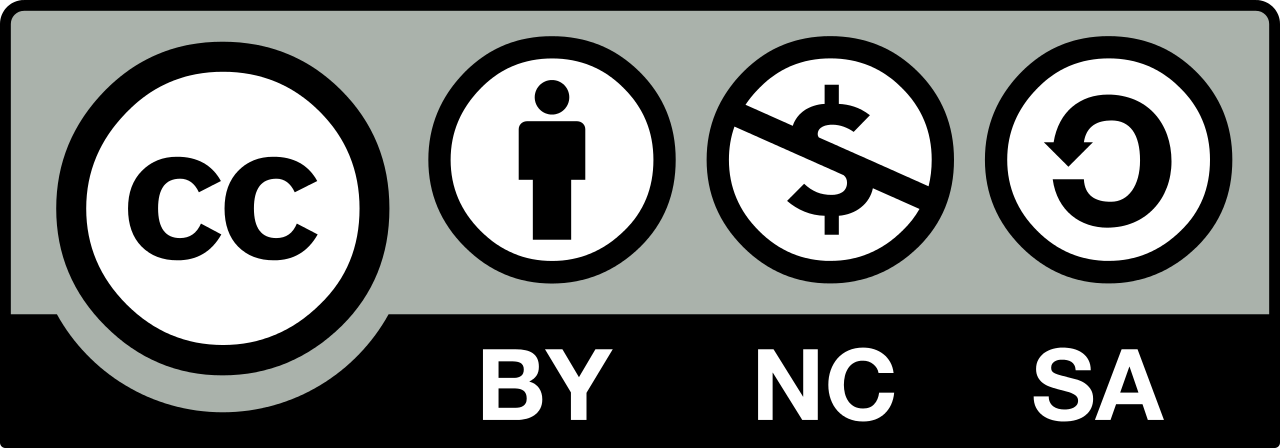
\includegraphics[width=3.5cm]{cc-by-nc-sa.png}
\end{minipage}\hfill
\begin{minipage}[c]{5cm}
\centering
{\large Desenvolvido por}


\includegraphics[width=2.5cm]{logo-associacao.jpg}
\end{minipage}
\begin{minipage}[r]{5cm}
\centering

{\large Patrocínio:}
  \vspace{1em}
  
\includegraphics[width=3.5cm]{itau}
\end{minipage}
\end{figure}

\mainmatter

\explore{O problema do cartógrafo}\label{cart_1}
Alguns autores afirmam que a Cartografia (do grego \textit{chartis} = mapa e \textit{graphein} = escrita) é, ao mesmo tempo, ciência e arte.  A arte é evidente, pois está associada à estética, clareza, harmonia e simplicidade. Especialmente em velhos mapas históricos (\hyperref[mapa_ant]{figura \ref{mapa_ant}}), nos quais quem o fazia, preenchia os oceanos com figuras de velhos barcos a vela, e outros tipos de desenhos.

\begin{figure}[H]
\centering
\includegraphics[height=66mm]{{mapa_ant}.png}
\caption{Mapa antigo. \\ Figura de \href{https://stock.adobe.com/br/images/old-vintage-world-map/178102789}{pingebat, no Adobe Stock}}
\label{mapa_ant}
\end{figure}


Já a cartografia como ciência vem do conhecimento de como comunicar, ou seja, quais instrumentos e técnicas devem ser utilizados para que a realidade seja representada com maior exatidão, ou seja, depende de conceitos da Astronomia e da Matemática. 
Assim, o cartógrafo (profissional dedicado à cartografia e à produção de mapas) precisa conhecer aspectos artísticos e técnicos para realizar seu trabalho.

Nas atividades a seguir, vamos pensar um pouco sobre o que esse profissional precisa conhecer para fazer uma representação plana da superfície do planeta Terra.

\clearpage

\begin{task}{O astronauta}\label{astronauta}
Descreva a cena ilustrada na \hyperref[carto1]{figura \ref{carto1}} a seguir

\begin{figure}[H]
\centering
\includegraphics[width=300bp]{{carto1}.jpg}
\caption{O astronauta. \\ Foto de \href{https://unsplash.com/photos/yEauzeZU6xo}{Monica Garniga, no Unsplash}}
\label{carto1}
\end{figure}

\begin{enumerate}
\item Faça um esboço que ilustre o que você descreveu.
\item Desenhe onde você está nesse esboço.
\item Sinalize onde estão as nuvens no seu esboço.
\end{enumerate}
\end{task}


\begin{task}{Qual o verdadeiro formato do planeta Terra?}
\label{forma_terra}

\textbf{Parte 1:} Será que o aplicativo que traça rotas entre dois pontos do planeta Terra pode estar errado? Observe os  mapas ilustrados nas \hyperref[rota1]{figuras \ref{rota1} e \ref{rota2}}  e responda as questões abaixo para auxiliar a desvendar este mistério!

\begin{figure}[H]
\centering
\includegraphics[width=0.8\textwidth]{{carto_2}.png}
\caption{Rota 1}
\label{rota1}
\end{figure}

\begin{figure}[H]
\centering
\includegraphics[width=0.8\textwidth]{{carto_3}.png}
\caption{Rota 2}
\label{rota2}
\end{figure}

A primeira  rota traçada no aplicativo, possui comprimento aproximado de 18.883 km (dezoito mil, oitocentos e oitenta e três quilômetros), já a segunda rota tem um  comprimento aproximado de 6.192 km (seis mil, cento e noventa e dois quilômetros).

\begin{enumerate}
\item Apenas observando as imagens é possível perceber que que a origem e o destino final dos dois mapas são iguais ou, pelo menos, muito semelhantes. Justifique  por que distância  entre estes dois pontos é tão distinta?
\item Seria possível chegar no destino final por outra rota (justificando a diferença de medidas)? Qual seria essa rota alternativa?
\item Mesmo sendo origem e destinos diferentes, você acha que a primeira é cerca de três vezes maior? Justifique sua resposta!
\item A representação está equivocada? Se sim, como seria a correta?
\end{enumerate}


\textbf{Parte 2:}
Na sua opinião, qual das imagens ilustradas na \hyperref[planeta]{figura \ref{planeta}} melhor representa o formato do planeta Terra? Por quê?

\begin{figure}[H]
\centering
\includegraphics[width=0.8\textwidth]{{carto4a}.jpg}
\caption{Representações da forma do planeta Terra}
\label{planeta}
\end{figure}

\end{task}

\begin{task}{Observando a paisagem}
Na \hyperref[paisag]{figura \ref{paisag}}  três homens estão observando a mesma paisagem. Observe que cada um deles está fazendo suas próprias combinações da arte e da ciência? Você concorda com essa afirmação? Justifique!

\begin{figure}[H]
\centering
\includegraphics[width=0.8\textwidth]{{carto10}.png}
\caption{Observando a paisagem \\ Fonte: \textbf{Anderson (1982)} }
\label{paisag}
\end{figure}


\end{task}



\arrange{O problema do cartógrafo}
\label{organizando-carto}
Ao observar a \hyperref[paisag]{figura \ref{paisag}}  é possível pensar que o escritor (pessoa situada no centro da figura) precisa conhecer as normas (a ciência) da construção gramatical e redação. Ou seja, o que ele faz é ciência? Alguns podem dizer que é arte, pois como escritor, é necessário realizar uma seleção das palavras, para a expressar verbalmente aquilo que ele percebe visualmente.

O pintor é um artista, por natureza. Porém, provavelmente ele aprendeu nas escolas de arte que estudou, os aspectos científicos das tintas, sobre os corantes, a respeito da combinação das cores, como perceber o ambiente, etc. 	
	
A terceira pessoa, pode ser um geógrafo, cartógrafo ou topógrafo. Nesse caso, como cientista, as medições que está realizando são muito importantes. Contudo, está aproveitando seu senso de estética para produzir um mapa, que é uma representação plana reduzida de uma dada área do espaço geográfico, que nesse caso, será ao mesmo tempo um resultado artístico e científico.

Observa-se que na cartografia, a arte inclui o esquema ou o \textit{layout} do desenho, que influi na aparência estética do mapa como um todo. Já a ciência inclui o conhecimento de quais símbolos colocar em um mapa e quais itens omitir e a noção da projeção a ser utilizada em cada situação. Ou seja, os mapas são uma expressão da necessidade humana de conhecer e representar o seu espaço e como produtos da cartografia, possuem algumas características importantes. Os mapas são imagens gráficas bidimensionais, resultado da aplicação de símbolos gráficos, como cores, ícones, pontos, linhas e outros. 

Alguns desses símbolos gráficos apresentam padronizações, como por exemplo, utilizar a cor azul para representar o mar, utilizar linhas tracejadas para representar ferrovias, aviões para representar aeroportos, etc.  O mar, as ferrovias, os aeroportos são aspectos retratados no mapa em uma determinada escala. 

Por isso, pensamos na atividade “\hyperref[astronauta]{O astronauta}”. Como você descreveu a imagem? Precisou pensar no planeta terra para descrevê-la? E ao fazer o esboço, o planeta terra precisou aparecer? Em que momento? Por quê?
Algumas pesquisas mostram que existem diferentes concepções das como representar o espaço que vivemos e essas noções podem depender da idade da pessoa ( \textbf{Nussbaum e Novick, 1979; Scheeren et al, 2016}).

Assim como existem diferentes representações da nossa percepção quanto ao lugar que ocupamos no espaço, isso pode influenciar na maneira que percebemos qual a forma que o planeta que vivemos possui. 
Essa preocupação em descrever a verdadeira forma da Terra, apesar de atualmente ser um assunto recorrente, remonta a Grécia antiga. O principal motivo, naquela época, para esta inquietação estava relacionado com a necessidade de compreender o mundo. 

Por volta do ano 200 antes da era Cristã, um matemático e astrônomo grego chamado Erastóstenes determinou a circunferência terrestre, comprovando, de certa forma que a Terra realmente possuía o formato de uma superfície esférica (\hyperref[esf]{figura \ref{esf}}), como é explicado na introdução do Capítulo de Trigonometria. 


\begin{figure}[H]
\centering
\includegraphics[width=0.3\textwidth]{{carto12}.jpg}
\caption{Modelo esférico da Terra. \\ Foto de \href{https://unsplash.com/photos/yEauzeZU6xo}{The New York Public Library, no Unsplash}}
\label{esf}
\end{figure}

No século XVII o físico inglês Isaac Newton e o matemático holandês Christiaan Huygens alegaram que a superfície terrestre não era esférica pois, possuía um sutil achatamento nos polos. Em função dessa descoberta, passou-se a considerar que a superfície da Terra não é uma esfera perfeita, mas que a figura geométrica mais semelhante a superfície do nosso planeta era o elipsoide de revolução. Um elipsoide de revolução é um sólido geométrico gerado por uma curva (chamada elipse) que gira  em  torno  do  seu  eixo  menor (\hyperref[elipse]{figura \ref{elipse}}).  

\begin{figure}[H]
\centering
\includegraphics[width=0.45\textwidth]{{carto11}.png}
\caption{Elipsoide de revolução. \\ Fonte: \href{Geogebra}{https://www.geogebra.org/m/dbu5h92x}} 
\label{elipse}
\end{figure}

Porém, pesquisas realizadas no final do séc. XIX e início do séc. XX eliminam a hipótese da superfície terreste ser um elipsoide de revolução, pelo contrário, chegou-se à conclusão de que a superfície da Terra possui muitas irregularidades e desta forma, seu formato não tem uma representação matemática muito simples. Buscando contornar esta falta de representação matemática explícita para a superfície da Terra, Johann Carl Friedrich Gauss, matemático alemão, caracterizou o geoide (\hyperref[geoide]{figura \ref{geoide}}. 

\begin{figure}[H]
\centering
\includegraphics[width=0.35\textwidth]{{carto5}.jpg}
\caption{Geoide. \\ Fonte: \href{https://apod.nasa.gov/apod/ap141215.html}{Astronomy Picture of The Day, Nasa}} 
\label{geoide}
\end{figure}


O geoide é um sólido muito parecido com a esfera com suaves ondulações e achatado nos polos.


Para fins didáticos, utiliza-se o o globo terrestre (\hyperref[globo]{figura \ref{globo}}), que é a representação da superfície da Terra  em uma esfera de tamanho reduzido. No site do Norman B. Leventhal Map \& Education Center \url{https://www.leventhalmap.org/digital-exhibitions/bending-lines/interactives/shaded-globe/} encontra-se uma versão digital do globo terrestre.


\begin{figure}[H]
\centering
\includegraphics[width=0.4\textwidth]{{carto13}.png}
\caption{Globo terrestre. \\ Foto de \href{https://unsplash.com/photos/9tmrYLRL7Ww}{Subhash Nusetti, no Unsplash}} 
\label{globo}
\end{figure}

Em termos cartográficos, em geral, assume-se uma escala média de 1 para 5.000.000, ao representar a Terra como uma esfera.

\begin{reflection}
Por que os corpos celestes (sol, lua e planetas, por exemplo) parecem ser todos aproximadamente esféricos? 
\end{reflection}



Mas, para produzir um mapa, necessitamos de alguns elementos já estudados na disciplina de Geografia, e é sobre isso que trata a próxima seção.



\begin{reflection}
Na atividade "\hyperref[forma_terra]{Qual o verdadeiro formato do planeta Terra?}" apresentamos sete imagens, discutimos sobre três. E as outras imagens, também podem ser representações da superfície da Terra?
\end{reflection}


\explore{Coordenadas Geográficas}\label{coord_geo}

\begin{task}{Que números são esses?}

\textbf{Parte 1}: Para realizar essa atividade é necessário o uso do aplicativo Google Maps (\url{https://www.google.com/maps})
\begin{enumerate}
\item Pesquise no aplicativo a sua cidade.
\item Clique ou toque em um ponto qualquer da cidade (insira um “alfinete”). Ao fazer isso, aparecerão alguns números na tela.
\item Copie esses números no seu caderno.
\item O que esses números significam?
\end{enumerate}

\textbf{Parte 2}: Para realizar essa atividade é necessário o uso do aplicativo Geogebra (\url{https://www.geogebra.org/m/fzcrw7nm}).
\begin{enumerate}
\item Movimente os controles deslizantes latitude e longitude, até obter os números obtidos na Parte 1, (despreze os números após o ponto).
\item Se a ordem dos números for trocada, o que ocorre?
\item Se o sinal for desprezado, o que ocorre?
\item Qual a relação dos valores “latitude” e “longitude” para os números obtidos na Parte 1?
\end{enumerate}

\end{task}


\arrange{Coordenadas Geográficas}
\label{organizando-coord_geo}

Para se determinar uma distância, ou um local qualquer sobre a superfície da Terra, é necessário sempre conhecer alguns elementos básicos. Um sistema de localização, por exemplo, composto pelo nome do Estado, da cidade, do bairro, da rua, número do prédio e do apartamento é suficiente para localizar uma pessoa que habita algum espaço urbano. 

Mas, se essa pessoa habita um espaço plano sem referências, surgirão obstáculos que impedem a materialização matemática de um sistema assim descrito, ou seja, dificultando sua representação em forma matemática. Para que isso aconteça, é preciso definir um sistema de coordenadas conveniente para registrar uma posição no espaço, qualquer que seja a dimensão que se esteja referenciando.  

Na  atividade “que números são esses?” Percebemos que existem números associados a diferentes locais da superfície terrestre. Mas de onde eles surgem?
Para representar a posição de um ponto sobre uma superfície (elipsóide, esfera ou plano) usar um sistema de coordenadas é indispensável. Para o plano, um sistema de coordenadas cartesianas $x$ e $y$ é usualmente aplicável, enquanto que para o elipsóide ou a esfera, usualmente empregamos um sistema de coordenadas cartesiano e curvilíneo.

Assim, para que cada ponto da superfície da Terra pudesse ser localizado no mapa, foi criado um sistema de linhas imaginárias chamado Sistema de Coordenadas Geográficas. Existem dois tipos de linhas imaginárias nos mapas e no globo terrestre, os paralelos e os meridianos (\hyperref[parmer]{figura \ref{parmer}}), que foram criados para facilitar/determinar a localização precisa de qualquer ponto na superfície da Terra. 


\begin{figure}[H]
\centering
\includegraphics[width=0.75\textwidth]{{carto21}.png}
\caption{Paralelos e meridianos}
\label{parmer}
\end{figure}

Os paralelos são linhas imaginárias que dão uma volta completa em torno da terra no sentido leste- oeste (\hyperref[paralelos]{figura \ref{paralelos}}).

\begin{figure}[H]
\centering
\includegraphics[width=0.3\textwidth]{{carto22}.png}
\caption{Paralelos e meridianos}
\label{paralelos}
\end{figure}

O principal paralelo, chama-se equador. A linha do Equador é o paralelo de referência, correspondendo ao círculo máximo perpendicular ao eixo da Terra e dividindo-a em dois hemisférios, Norte e Sul. Os restantes dos paralelos são círculos menores paralelos ao Equador. Além do Equador, outros paralelos conhecidos são o trópico de câncer, o trópico de capricórnio, o círculo polar ártico e o círculo polar antártico (\hyperref[ppar]{figura \ref{ppar}}).

\begin{figure}[H]
\centering
\includegraphics[width=0.4\textwidth]{{carto23}.png}
\caption{Principais paralelos}
\label{ppar}
\end{figure}

\begin{knowledge}
A cidade de Macapá  é a única capital do Brasil cortada pela linha do Equador? Lá existe um estádio de futebol chamado Zerão cuja linha central do meio de campo é a linha imaginária do Equador, assim um time joga no hemisfério Norte e outro no hemisfério Sul. Interessante, né?  
\end{knowledge}
 
Os meridianos são linhas imaginárias que cortam a Terra do polo norte ao polo sul. Eles são círculos máximos que passam pelos polos e são perpendiculares ao Equador. A metade de um meridiano que vai de pólo a pólo chama-se  semi meridiano. O meridiano de referência, que divide a Terra em oeste e leste,  adotado desde 1884 é o semi meridiano de Greenwich (\hyperref[mer]{figura \ref{mer}}) , que passa pelo observatório astronômico de mesmo nome na Grã Bretanha.

\begin{figure}[H]
\centering
\includegraphics[width=0.35\textwidth]{{carto24}.png}
\caption{Meridianos}
\label{mer}
\end{figure}

 
A coordenada geográfica de um determinado ponto da superfície da Terra é obtida pela interseção de um meridiano e um paralelo. Assim, em um sistema de coordenadas geográficas, cada ponto na superfície da Terra é identificado por dois ângulos (expressos habitualmente em graus, minutos e segundos): longitude ($\phi$) e a a latitude ($\lambda$ ) (\hyperref[latlon]{figura \ref{latlon}}).


\begin{figure}[H]
\centering
\includegraphics[width=0.4\textwidth]{{carto25}.png}
\caption{Latitude e longitude}
\label{latlon}
\end{figure}


A latitude de um lugar é a amplitude do ângulo entre o plano do Equador e o raio que passa por esse lugar ou o arco do meridiano entre o Equador e o lugar. a latitude varia de $0^{\circ}$, no Equador a $90^{\circ}$ nos polos Norte (N) ou Sul (S).   A latitude quando medida no sentido do polo Norte é chamada Latitude Norte ou Positiva, quando medida no sentido Sul é chamada Latitude Sul ou Negativa. 

E a longitude de um lugar é a amplitude do ângulo entre o plano do meridiano desse lugar e o semimeridiano de Greenwich ou o arco do Equador entre esses meridianos. Ela varia entre $0^{\circ}$ e $180^{\circ}$ Este (E) ou Oeste (W). A longitude pode ser medida no sentido oeste, quando é chamada Longitude Oeste de Greenwich  ou Negativa. Se medida no sentido este, é denominada Longitude Este de Greenwich ou Positiva.

Os valores de latitude e longitude de um local determinam as coordenadas geográficas do mesmo 

Por exemplo, a cidade do Rio de Janeiro está localizada a uma latitude de aproximadamente $22^{\circ}$ S  e uma longitude aproximada de $43^{\circ}$ W (\hyperref[rio]{figura \ref{rio}}).

\begin{figure}[H]
\centering
\includegraphics[width=0.7\textwidth]{{carto26}.png}
\caption{Rio de Janeiro}
\label{rio}
\end{figure}
 

E a cidade de Nova Iorque situa-se a uma latitude de aproximadamente $41^{\circ}$ N  e uma longitude aproximada de $74^{\circ}$ O (\hyperref[nova]{figura \ref{nova}})

\begin{figure}[H]
\centering
\includegraphics[width=0.7\textwidth]{{carto27}.png}
\caption{Nova Iorque}
\label{nova}
\end{figure}

 
O vídeo \url{https://youtu.be/ibE2S8OkNJ8} apresenta mais detalhes sobre essas coordenadas.

Na próxima seção vamos observar algumas deformações que ocorrem quando "passamos" da superfície esférica ( globo terrestre, por exemplo) para o mapa.

\begin{knowledge}
\begin{itemize}
\item Para localizar com maior precisão um ponto na superfície terrestre, além das coordenadas geográficas, podemos utilizar uma outra informação, o nível do mar. Altitude é diferente de altura, que é a dimensão vertical de um corpo da base até seu ponto extremo.

\item O GPS (sigla em inglês para sistema de posicionamento global) é atualmente o grande recurso para se localizar um ponto na superfície da Terra. No mostrador do aparelho aparecem as coordenadas e a altitude do local, obtidas através de sinais enviados por um conjunto de satélites (24 satélites). É esse sistema acoplado aos aviões de combate que permite atingir o alvo desejado com grande precisão, como, por exemplo, na Guerra dos EUA contra o Afeganistão. No Brasil, tal sistema é utilizado pelo IBGE (Instituto Brasileiro de Geografia e Estatística) para orientação aérea, terrestre e marítima, passando também a equipar veículos para navegação terrestre.
\end{itemize}
\end{knowledge}





\explore{Mapas e rotas}\label{mapamundo}
Um mapa do mundo (ou mapa-múndi) é uma maneira de retratar a Terra como superfície esférica em um pedaço plano de papel. Para pequenas áreas, a superfície da Terra é muito semelhante a uma folha plana e, portanto, é mais simples desenhar com precisão as características geográficas dessa área, mantendo as distâncias precisas.

Se estivermos interessados em mapear uma área muito maior, ou talvez até o próprio mundo inteiro, como podemos fazer?

\begin{task}{Planificando o globo} \label{balao}

Vamos simular a planificação da superfície do planeta Terra utilizando um balão. Para isso você vai precisar de uma tesoura (sem ponta), um balão e uma caneta esferográfica. Também é recomendado que você tenha um pedaço de papelão (com tamanho igual a metade de uma folha A4) e fita adesiva.
Para realizar essa atividade, precisamos que você encha um pouco o balão, deixando-o mais próximo possível de uma esfera. Talvez necessite molda-lo com as mãos. Quando atingir o formato desejado de um nó na “boca” do balão. Ao finalizar essa etapa da atividade deve ter em mãos um balão como o ilustrado na \hyperref[balao1]{figura \ref{balao1}}.


\begin{figure}[H]
\centering
\includegraphics[width=0.4\textwidth]{{bala1}.png}
\caption{Balão}
\label{balao1}
\end{figure}


Com a caneta esferográfica solte sua criatividade e desenhe sobre o balão, procure deixar imagens bem definidas para melhor observação, como ilustra a \hyperref[balao2]{figura \ref{balao2}}.

\begin{figure}[H]
\centering
\includegraphics[width=0.4\textwidth]{{bala2}.png}
\caption{Balão com desenhos}
\label{balao2}
\end{figure}

Agora é necessário furar o balão. Mas, tenha muita atenção e cuidado para não o estourar. Para isso, você deve pegar o mais próximo da ponta do balão, e fazer um pequeno furo para que o ar saia do interior do balão, sem que ele estoure. Precisamos também desprezar o nó (\hyperref[balao3]{figura \ref{balao3}}), por isso corte-o, será mais fácil trabalhar sem ele.
 

\begin{figure}[H]
\centering
\includegraphics[width=0.4\textwidth]{{bala3}.png}
\caption{Cortando o nó}
\label{balao3}
\end{figure}

Tente deixar o balão esticado sobre uma superfície plana (o papelão), com todos desenhos para cima. Você pode cortar e esticar ou fazer outra ação que você julgar necessário. Use a  fita durex, ela será  útil nesse processo.
Agora, responda as questões:
\begin{enumerate}
\item Foi simples esticar o balão?
\item Para que ele ficasse plano, foi necessário realizar algum corte ou esticá-lo?
\item Perceba como ficaram as figuras desenhadas anteriormente, anote em seu caderno suas conclusões para compartilhar com os colegas.
\end{enumerate}

\end{task}



\begin{task}{Mapa e Globo} \label{mapa_globo}

Já sabemos o que são mapas e globos. A \hyperref[mapaglobo]{figura \ref{mapaglobo}} ilustra um globo (a direita) e um mapa ( à esquerda) 
Se traçarmos algumas rotas entre duas cidades no  globo, como será que ela irá se comportar no mapa? Ou seja, quais são as diferenças no traçado das rotas no mapa e no globo?

\begin{figure}[H]
\centering
\includegraphics[width=0.8\textwidth]{{carto15}.png}
\caption{Mapa e globo}
\label{mapaglobo}
\end{figure}

Para realizar a atividade recomendamos o uso do Geogebra (\url{https://www.geogebra.org/m/qvzrwuma})

\begin{enumerate}
\item Movimente os pontos vermelhos sobre o globo e observe a rota que foi traçada.
\item O que você percebe?
\item Habilite a caixa cilindro, localize um dos pontos no sul do continente Americano e o outro ponto no norte do continente Europeu. A rota que aparece no globo é a mesma do mapa? Justifique !
\end{enumerate}

\end{task}

\begin{task} {O caminho mais curto} \label{caminho}

Para realizar essa atividade é necessário o uso do aplicativo Geogebra (\url{https://www.geogebra.org/material/edit/id/30387421}) (\hyperref[rota3]{figura \ref{rota3}})

\begin{figure}[H]
\centering
\includegraphics[width=0.4\textwidth]{{carto_28}.png}
\caption{A menor rota.}
\label{rota3}
\end{figure}


Aparentemente a rota traçada em cor de rosa parece mais curta que a rota traçada em verde. 
Com o ponto amarelo, é possível alterar a rota traçada em rosa sobre o globo, mas observe que ela nunca será ser mais curta que a rota traçada em verde. Por que isso acontece?

\end{task}


\arrange{Mapas e Rotas}
\label{organizando-mapa}

 
Os cartógrafos, navegadores e outros que precisam de mapas planos para usos práticos, há muito tempo têm sido desafiados a mostrar a Terra, uma esfera tridimensional, em um plano e bidimensional, como foi simulado na atividade \hyperref[balao]{Planificando o globo}.

Outra forma de perceber o quanto é complexo realizar essa transformação, seria descascar uma laranja, tentando da melhor maneira possível manter a casca com apenas uma corte. Depois “planificar a casca”, ou seja, tentar  coincidir a casca da laranja com a superfície plana da mesa (\hyperref[laranja]{figura \ref{laranja}}). Para alcançar um contato total entre as duas superfícies, a casca de laranja teria que ser distorcida (quebraria   assim como ocorreu com o balão.

\begin{figure}[H]
\centering
\includegraphics[width=0.6\textwidth]{{laranja}.png}
\caption{Laranja planificada.  \\ Fonte: \href{https://www.pngkey.com/maxpic/u2r5u2a9u2o0a9r5/}{pngkey}}
\label{laranja}
\end{figure}

O fato que qualquer representação plana que se faça da superfície terrestre  sempre possuir algum tipo de distorção, é uma consequência do Teorema Egregium (do Latim “notável”)  provado  pelo matemático alemão Johann Carl Friedrich Gauss (1777-1855).
Em particular, a superfície de uma esfera não pode ser representada  em um plano sem nenhuma distorção. Esse fato foi  provado matematicamente, pelo físico  matemático Leonhard Paul Euler no século XVIII (veja \hyperref[Euler1]{\textit{Para Saber Mais: Euler e a Superfície Terrestre}}).

 Mas, desde os anos 1500, matemáticos têm tentado criar algoritmos que poderiam transformar o globo em algo plano. Pra fazer isso, eles usam um processo chamado projeção cartográfica. 

As projeções cartográficas são técnicas essenciais para a cartografia e compõem o sistema que serve de base para criação dos mapas. Essas técnicas consistem na representação do globo (ou parte dele) em uma superfície plana.

Na atividade \hyperref[mapa_globo]{Mapa e o Globo}, podemos observar que as rotas são diferentes no globo e no mapa. Por exemplo, se escolhermos como ponto de partida a ilha de Madagascar no continente Africano e como ponto de chegada o norte  Russia é possível perceber uma distorção muito grande da rota no globo para a rota no mapa.  Mas, ao habilitar o cilindro, é possível visualizar a curva do globo projetada no cilindro (curva pontilhada) que é exatamente a mesma curva no mapa(\hyperref[globomapa1]{figura \ref{globomapa1}}).


\begin{figure}[H]
\centering
\includegraphics[width=0.8\textwidth]{{carto16}.png}
\caption{Rotas}
\label{globomapa1}
\end{figure}

Já na atividade \hyperref[caminho]{O caminho mais curto} se colocarmos os pontos $A$ e $B$ no mesmo paralelo, é possível conjecturar que uma rota ao longo deste círculo, unindo esses dois pontos seria a mais curta possível (\hyperref[rota4]{figura \ref{rota4}}).

\begin{figure}[H]
\centering
\includegraphics[width=0.6\textwidth]{{carto31}.png}
\caption{Rotas.}
\label{rota4}
\end{figure}
 
Porém essa rota não é a mais curta. A rota mais curta entre dois pontos da superfície esférica está sempre sobre um círculo máximo, que é aquele cujo centro coincide com o centro da esfera. Essa rota é em geral designada por ortodromica ou por rota de grande círculo. Tem uma utilidade prática, pois é aquela que, de forma aproximada, é percorrida pelas aeronaves e navios em viagens de longo curso.

Assim, podemos dizer que um círculo máximo  é um círculo de maior diâmetro que pode ser traçado sobre a superfície de uma esfera. Esse círculo tem a propriedade de dividir a terra em dois hemisférios iguais. O equador é um exemplo de círculo máximo. 

Agora que já conhecemos as coordenadas geográficas, sabemos que é impossível planificar uma esfera em um plano se realizar distorções e que as rotas traçadas na superfície plana se comportam de forma diferente na superfície esférica, podemos pensar como são as distorções que ocorrem nas projeções cartográficas e como os paralelos e meridianos se comportam, e como são as rotas mais curtas em cada projeção, por exemplo.

\know{Euler e a superfície terrestre}{\label{Euler1}

No século XVII Euler demonstrou o seguinte fato: A superfície de uma esfera não pode ser representada  em um plano sem nenhuma distorção. A demonstração realizada foi a seguinte:
Considerando uma pequena região ao redor de um ponto $P$ da esfera de raio $r$. Seja também um ponto $Q$ sobre a esfera, com $ \widehat{PQ} = l$ . Uma circunferência de raio $s$ pode ser formada por todos os pontos que distam $l$ de $P$ na esfera conforme a \hyperref[euler]{figura \ref{euler}}.

\begin{figure}[H]
\centering
\includegraphics[width=0.4\textwidth]{{euler}.png}
\caption{Região da esfera ao redor do ponto $P$}
\label{euler}
\end{figure}

Supondo que os pontos da esfera possam ser representados em um plano por um fator de escala $m$ e assim sendo, o arco de comprimento $l$ ao longo de um grande círculo da esfera seria transformado num segmento retilíneo de comprimento $l$ vezes um fator de escala $m$ no mapa plano. Assim, todos os pontos que equidistam $l$ de $P$ na esfera deveriam ser mapeados por pontos que distam de $ml$ de $P$ no plano. 

A nova circunferência obtida no plano teria comprimento $2\pi 𝑚l$. Por outro lado, os pontos $Q$ na esfera com $ \widehat{PQ} = l$, formariam uma circunferência de raio $s$ com $s < l$, pois da Geometria Elementar, temos que o comprimento do arco $l$ é igual ao produto do raio da circunferência pelo ângulo, ou seja, $l = \alpha r$ e conforme a \hyperref[euler]{figura \ref{euler}} temos que $s =r \sin (\alpha)$. Como $\alpha > \sin(\alpha)$ resulta que $s < l$.

Desta forma, o comprimento da circunferência de raio $s$ representado no plano a um fator de escala $m$ seria $2\pi 𝑚𝑠$ que é menor que $2\pi 𝑚l$. Não podemos ter uma imagem com circunferência de comprimento igual a $2\pi 𝑚l$ e menor que $2\pi 𝑚l$ ao mesmo tempo, o que nos conduz a uma contradição e conclui a demonstração.

Fonte: \textbf{Ávila(2008)}


\explore{Um mapa para o mundo}\label{mapamundo1}

\begin{task}{Observando os mapas}\label{obs_mapas}

\textbf{Parte 1: } Observe o mapa ilustrado na \hyperref[meca]{figura \ref{meca}} e  responda as questões abaixo:

\begin{figure}[H]
\centering
\includegraphics[width=0.5\textwidth]{{meca}.png}
\caption{Projeção Cartográfica Mercartor. \\ Fonte: \href{https://map-projections.net/}{Compare Map Projections}}
\label{meca}
\end{figure}

\begin{enumerate}
\item Você acredita que a área correspondente aos continentes está correta?
\item Compare a área da Groelândia e da América do Sul no mapa. Isso corresponde à realidade? Justifique!
\item Compare a área do continente europeu ao do continente africano. Isso corresponde à realidade?
\item Preste atenção nas linhas de latitudes (horizontais) elas têm 10º de diferença, ou seja, na superfície de uma esfera, tem a mesma distância. Utilize disso para argumentar o porquê das suas respostas anteriores.

\end{enumerate}

\textbf{Parte 2:}  O mapa ilustrado na  \hyperref[meca]{figura \ref{meca}} é o utilizado pelo aplicativo \textit{The True Size}. Utilize o site   \url{https://thetruesize.com} para comparar o tamanho dos países indicados abaixo. Caso selecione algum pais de forma equivocada, clique com o botão direito do mouse para limpar a seleção ou clique em \textit{Clear map}. Para comparar os países, basta colocar o nome de cada um deles no espaço anterior a lupa, como ilustra a \hyperref[true]{figura \ref{true}}.

\begin{figure}[H]
\centering
\includegraphics[width=0.3\textwidth]{{true}.png}
\caption{Fonte: \href{https://thetruesize.com}{The True Size}}
\label{true}
\end{figure}
 
 \begin{enumerate}
\item Selecione no mapa o Brasil (Brazil) e a Groelandia (Greenland). Arraste a Groelandia para o lugar do Brasil. Observe o que acontece! Por que isso ocorre? 
\item Faça o mesmo para a Bolívia e a Alemanha (Germany)
\item Você percebe que a África, o sul da Ásia e América do Sul parecem muito menores em relação aos países mais distantes do equador? Por que isso ocorre?

\end{enumerate}


\textbf{Parte 3:} Observe o mapa ilustrado na \hyperref[peters]{figura \ref{peters}} e responda as questões abaixo.

\begin{figure}[H]
\centering
\includegraphics[width=0.5\textwidth]{{peter}.png}
\caption{Projeção Cartográfica Gall-Peters.  \\ Fonte: \href{https://map-projections.net/}{Compare Map Projections}}
\label{peters}
\end{figure}

\begin{enumerate}
\item	Você acredita que a área correspondente aos continentes está correta?
\item Compare a área da Groelândia e da América do Sul no mapa. Isso corresponde à realidade? Justifique!
\item Compare a área da América do Norte a do continente africano. Isso corresponde à realidade?
\item Quais dos dois mapas você escolheria para representar a superfície do planeta Terra? Por quê?
\item Preste atenção nas linhas de latitudes (horizontais) elas têm 10º de diferença, ou seja, na superfície de uma esfera, tem a mesma distância. Utilize disso para argumentar o porquê das suas respostas anteriores.
\end{enumerate}
\end{task}


\arrange{Um mapa do mundo}
\label{organizando-mapa1}

Os mapas apresentados nas \hyperref[meca]{figuras \ref{meca} e \ref{peters}}, em particular, são representações cartográficas planas, em escala reduzida, de toda a superfície do planeta Terra . Mapas com essa característica são denominados mapa-múndi ou planisfério. 
Existem diferentes maneiras de projetar a superfície da Terra em um mapa plano (a partir de um cilindro, por exemplo); no entanto, um problema permanece: não é possível mostrar a Terra com precisão. Mas mesmo para  mostrá-la aproximadamente, somos forçados a esticar algumas partes da superfície, comprimir outras, talvez curvá-las um pouco. Isso leva a distorções. É importante observar que todo e qualquer mapa do mundo terá algum tipo de distorção!

A atividade \hyperref[obs_mapas]{Observando os mapas} explora um pouco dessas distorções. Observe que ambos os mapas-múndi apresentados tem formato retangular, isso ocorre porque ambos foram feitos utilizando uma projeção cartográfica do tipo cilíndrica. Mas como isso é feito? Imagine colocar um cilindro reto sobre o globo e projetar cada ponto da esfera, na superfície do cilindro, depois desenrolar o cilindro. Fazendo isso, obtemos um mapa plano e retangular. Nas próximas seções iremos abordar mais detalhes sobre esse assunto.  
Apesar de termos dois mapas retangulares e que representam a superfície da Terra, ao compará-los percebemos que existem algumas diferenças ( \hyperref[proje]{figura \ref{proje}}). 

\begin{figure}[H]
\centering
\includegraphics[width=0.8\textwidth]{{carto17}.png}
\caption{Diferentes projeções. \\ Fonte: Fonte: \href{https://map-projections.net/}{Compare Map Projections}}
\label{proje}
\end{figure}

O mapa da esquerda na \hyperref[proje]{figura \ref{proje}} denomina-se Projeção Mercator,  é um dos mapa-múndi mais famosos do mundo. Ele foi inventado no século XVI pelo cartógrafo flamengo Gerardus Mercator e  preserva a forma dos países. Por exemplo, o Brasil, no globo, tem a mesma forma do Brasil nesse mapa (\hyperref[brasil]{figura \ref{brasil}}).

\begin{figure}[H]
\centering
\includegraphics[width=0.8\textwidth]{{carto18}.png}
\caption{O Brasil na Projeção Mercator. \\ Fonte: \url{https://youtu.be/kIID5FDi2JQ}}
\label{brasil}
\end{figure}

Mas o verdadeiro propósito do mapa inventado por Mercator era a navegação. Esse mapa preserva a direção, o que é muito importante, por exemplo,  ao navegarmos no oceano com apenas uma bússola. 

O mapa da direita na \hyperref[proje]{figura \ref{proje}}, denominado  Projeção Cartogáfica Gall-Peters, possui esse nome pois foi construída originalmente por James Gall, um um clérigo (padre) escocês  em 1885, mas foi vastamente ignorada. Porém, foi resgatado em 1973 pelo historiador alemão Arno Petes. Esse mapa é um pouco controverso, pois preserva a área, mas as formas dos países estão totalmente distorcidas. Além disso, apresenta um cunho político, pois amplia de forma significativa  as áreas dos países do sul, que em sua maioria é subdesenvolvida, e diminui as áreas dos países do norte, de maioria desenvolvida. Nesse planisfério, a África é colocada no centro do mapa, ao contrário do mapa feito por Mercator, em que a Europa encontrava-se no centro.


\begin{knowledge}
Qualquer pessoa que goste muito de viajar, é capaz de perder horas e horas vasculhando o Google Maps. Mas até meados de 2018, quando o usuário reduzia o zoom para ver o planeta inteiro, o mundo era apresentado na Projeção Cartográfica Mercator. Atualmente, o Google Maps apresenta a superfície terrestre de forma tridimensional e esférica.
\end{knowledge}


Além os mapas citados, existem outros provenientes de projeções cilíndricas.  Por exemplo a projeção cilíndrica equidistante (\hyperref[cil_equi]{figura \ref{cil_equi}}), que foi projetada por Marinus de Tyre (por volta do ano 100 da era Cristã).

\begin{figure}[H]
\centering
\includegraphics[width=0.8\textwidth]{{carto19}.png}
\caption{Projeção Cilíndrica Equidistante. \\ Fonte: \href{https://map-projections.net/}{Compare Map Projections}}
\label{cil_equi}
\end{figure}

Outro exemplo é  o mapa  elaborado pelo cartógrafo e geógrafo norte-americano Arthur Robinson  na década de 1960 (\hyperref[rob]{figura \ref{rob}}.

\begin{figure}[H]
\centering
\includegraphics[width=0.8\textwidth]{{carto20}.png}
\caption{Projeção Cilíndrica de Robinson. \\ Fonte: \href{https://map-projections.net/}{Compare Map Projections}}
\label{rob}
\end{figure}

A grande vantagem dessa projeção em relação as demais, é que ela se encontra em um meio termo. Ela não preserva nem a forma e nem a correta área dos continentes. No entanto, ela consegue minimizar as distorções que ocorrem nesses dois aspectos.

Observando os exemplos citados acima,  percebemos um problema, cada uma dessas  projeções cartográficas,  têm sua própria configuração de forma, distância, direção e área. Portanto, é importante reconhecer que as projeções cartográficas sempre possuem algum tipo de distorção. Além disso, como não é possível se desenvolver uma superfície esférica sobre um plano sem deformações, na prática, os cartógrafos buscam projeções onde seja possível diminuir ou eliminar parte das deformações, dependendo de onde e para qual fim essa projeção cartográfica será utilizada. 
As projeções cartográficas, de acordo com o tipo de distorção são classificadas da seguinte forma: 



\begin{enumerate}
\item Equidistantes: Não apresentam deformações lineares, ou seja, os comprimentos são representados em escala uniforme.
\item Conformes: Representam sem deformação todos os ângulos em torno de quaisquer pontos, e dessa maneira, não deformam pequenas regiões.
\item Equivalentes: Conservam as áreas. Seja qual for a porção representada num mapa, ela conserva a mesma relação com a área de todo o mapa.
\item Equivalentes: Não possui nenhuma das propriedades dos outros tipos, isto é, equivalência, conformidade e equidistância, ou seja, as projeções em que as áreas, os ângulos e os comprimentos não são conservados.

\end{enumerate}

As propriedades acima descritas são mutuamente exclusivas. Isso reforça o fato de  que não existe uma projeção cartográfica ideal, mas apenas a melhor representação para um determinado propósito.

Um método muito utilizado  para visualizar as distorções de uma projeção cartográfica é a Indicatriz da Tissot ( que já foi apresentada no livro de Projeções e Perspectivas. Foi introduzido em 1859 pelo matemático francês Nicolas Auguste Tissot.
Esse método consiste no seguinte:  Imagine desenhar diversos círculos  de mesmo  tamanho, em intervalos regulares  na superfície da Terra. Feito isso, a Terra vista do espaço será como a ilustrada na \hyperref[tiss1]{figura \ref{tiss1}}.


\begin{figure}[H]
\centering
\includegraphics[width=0.4\textwidth]{{tiss 1}.png}
\caption{Círculos desenhados na superfície terrestre. \\ Fonte: \href{https://map-projections.net/}{Compare Map Projections}}
\label{tiss1}
\end{figure}


Ao projetar essa superfície em um plano, os círculos ficaram distorcidos. Essa distorção irá depender da projeção cartográfica escolhida. Por exemplo, na Projeção Mercator a indicatriz de Tissot está ilustrada na \hyperref[tiss2]{figura \ref{tiss2}}.

\begin{figure}[H]
\centering
\includegraphics[width=0.6\textwidth]{{tiss2}.jpg}
\caption{Indicatriz de Tissot – Projeção Mercator. \\ Fonte: \href{https://map-projections.net/}{Compare Map Projections}}
\label{tiss2}
\end{figure}
Podemos observar que os círculos mantiveram sua forma circular, mas ficam cada vez maiores conforme nos aproximamos dos polos.
E é exatamente isso que a projeção de Mercator faz: mantém as formas (localmente), mas faz com que diferentes regiões no mapa tenham tamanhos desproporcionais entre si.
O vídeo \url{https://www.youtube.com/watch?v=E43g5EMxaTg} apresenta como essas distorções surgem. 
 Em contraponto, podemos observar a indicatriz de Tissot na Projeção Robinson, que conforme dissemos,  minimiza as distorções .
 
 
\begin{figure}[H]
\centering
\includegraphics[width=0.6\textwidth]{{tiss3}.png}
\caption{Indicatriz de Tissot – Projeção Robinson. \\ Fonte: \href{https://map-projections.net/}{Compare Map Projections}}
\label{tiss2}
\end{figure} 
  

Algo que precisamos entender é como as projeções cartográficas são concebidas. É possível projetar o globo em  objetos como cilindros, cones e planos (figura xx), denominados superfícies de projeção. As caracteristicas desses objetos, juntamente com a matemática que a pessoa que está pensando,  vai afetar na aparência da projeção cartográfica resultante. 

\begin{figure}[H]
\centering
\includegraphics[width=0.8\textwidth]{{carto30}.png}
\caption{Possiblidades de projetar a esfera. \\ Fonte: \href{https://map-projections.net/}{Compare Map Projections}}
\label{tiss2}
\end{figure} 


Embora algumas projeções usem um processo geométrico, na realidade, a maioria das projeções usa processos analíticos (equações matemáticas) para transformar as coordenadas de um globo em uma superfície plana. Conforme visto anteriormente, historicamente os cartógrafos tiveram o desafio de representar a superfície curva da Terra em um plano e para esse fim, foram criadas as projeções cartográficas. 

Podemos dizer que uma projeção cartográfica é uma transformação da superfície da Terra (superfície de referência - SR) em uma superfície de projeção (SP),  por meio de expressões matemáticas. Durante essa transformação, os pontos que possuem coordenadas geográficas angulares (latitude, longitude) na superfície da Terra são convertidas em coordenadas cartesianas $(x, y)$ representando a posição dos pontos em um mapa plano. 
No nosso caso, trabalharemos com SP desenvolvíveis(cone, cilindro e plano) e para estabelecer as conexões entre as coordenadas da SR ( esfera) e as coordenadas cartesianas $(x,y)$ do plano de projeção precisamos encontrar as relações funcionais 
$x=f_1(\phi, \lambda)$ e $y=f_2(\phi, \lambda)$.

\begin{reflection}
Uma projeção cartográfica  pode ser interpretada como uma função  $f$ de domínio  $S^3$ (esfera, no nosso caso) e contradomínio $\pi$ (plano) que, a cada ponto $P \in S^3$  associa o ponto $P' \in \pi$. A expressão matemática associada, irá depender do tipo de projeção realizada.
\end{reflection}

\know{Para saber mais}
Uma projeção cartográfica  que possui uma dedução matemática simples é a a Projeção Cilíndrica Estereográfica de Braun. Essa projeção foi concebida por C.Braun e pode ser visualizada geometricamente da seguinte forma: a superfície de projeção é uma folha cilíndrica firmemente enrolada contra o Equador. Todo meridiano é atraído para este tubo por raios de luz que emanam de um ponto equatorial no meridiano diretamente oposto. O tubo tangente é então cortado ao longo de um meridiano arbitrário e desenrolado (\hyperref[cilindro]{figura \ref{cilindro}}).

\begin{figure}[H]
\centering
\includegraphics[width=0.6\textwidth]{{carto32}.png}
\caption{Projeção Cilíndrica. \\ Fonte: \url{https://progonos.com/}}
\label{cilindro}
\end{figure}


As equações para o mapeamento são simples. Consideremos projetar o ponto $P$ na Terra no ponto $P'$ no mapa.

Observemos que os meridianos nesse caso são projetados como linhas verticais retas com espaçamento diretamente proporcional à longitude $\phi$, portanto $x = R \phi$. 

O paralelo  é projetado como uma linha horizontal reta, cuja coordenada $y$  pode ser determinada observando os dois triângulos formados na \hyperref[triang]{figura \ref{triang}}. 

\begin{figure}[H]
\centering
\includegraphics[width=0.5\textwidth]{{carto33}.png}
\caption{Triâgulos}
\label{triang}
\end{figure}

Dai, temos
$$ \frac{h}{w+R} \frac{y}{2R}$$

E portanto, 

$$y=\frac{2Rh}{w+R}$$

Mas,

$$h=R \sin(\lambda)$$
$$w=R \cos(\lambda)$$

Portanto,

$$y=\frac{2R^2 \sin(\lambda)}{R \cos(\lambda)+R}=\frac{2R\sin(\lambda)}{\cos(\lambda) +1}$$

Fazendo $\theta=\frac{\lambda}{2}$ e usando as identidades trigonométricas $\sin(2\theta)=2\sin(\theta)\cos(\theta)$ e $\cos^2(\theta)=1-2\sin^2 (\theta)$, para  $\frac{-\pi}{2}\leq \lambda \leq \frac{\pi}{2}$, vem:

$$y=\frac{4R\sin(\theta)\cos(\theta)}{2(1-\sin^2(\theta)}= \frac{2R\sin(\theta)}{\cos(\theta)}=2Rtg(\theta).$$

Ou seja, para essa projeção, $$x = R\phi$$  $$y=2R \tan(\frac{\lambda}{2}).$$

A Projeção Cilíndrica Estereográfica de Braun possui o seguinte aspecto (\hyperref[braun]{figura \ref{braun}}).

\begin{figure}[H]
\centering
\includegraphics[width=0.6\textwidth]{{carto34}.png}
\caption{Projeção Cilíndrica Estereográfica de Braun. \\ Fonte: \href{https://map-projections.net/}{Compare Map Projections}}
\label{braun}
\end{figure}

\explore{Projeções Cilíndricas}\label{Pcilindricas}

\begin{task}{Projetando a esfera em uma superfície cilíndrica}\label{proj_cil}
Nessa atividade vamos simular uma projeção cartográfica do tipo cilíndrica. Para isso, serão necessários os seguintes materiais:
\begin{enumerate}
\item Tesoura (com ponta)
\item Lanterna (pode ser do celular)
\item Garrafa PET transparente 
\item Fita auto adesiva
\item Caneta esferográfica
\item Papel vegetal (ou papel manteiga)
\item Cola bastão
\end{enumerate}

Na garrafa pet, faça 3 cortes como ilustra a \hyperref[garrafa]{figura \ref{garrafa}} (o corte do bico é opcional)

\begin{figure}[H]
\centering
\includegraphics[width=0.4\textwidth]{{garrafa}.png}
\caption{Cortes na garrafa}
\label{garrafa}
\end{figure}

Com a caneta esferográfica desenhe (preferencialmente na parte interna) da parte A (\hyperref[garrafa1]{figura \ref{garrafa1}}), procure deixar figuras bem definidas para futuras observações.

\begin{figure}[H]
\centering
\includegraphics[width=0.4\textwidth]{{cilindro1}.png}
\caption{Desenhos na superfície da parte A da garrafa.}
\label{garrafa1}
\end{figure}
  

Forre a parte externa do cilindro (parte B da garrafa) com  o papel vegetal (ou manteiga ). Sugerimos que utilize um pouco de cola bastão e faça duas linhas verticais na parte B (de preferência em locais opostos) apenas o suficiente para que segurar o papel (\hyperref[cilindro2]{figura \ref{cilindro2}} – A). Lembre que posteriormente o papel deverá ser retirado. É possível também colar as extremidades do papel com fita adesiva (\ref{cilindro2} – B), mas esse processo pode danificar o papel.

\begin{figure}[H]
\centering
\includegraphics[width=0.4\textwidth]{{cilindro2}.png}
\caption{Formas de enrolar o cilindro.}
\label{cilindro2}
\end{figure}


Pegue a semiesfera (parte A) e o cilindro (parte B)  e coloque  semiesfera com os desenhos  “representação do mapa” como uma tampa do cilindro,  conforme ilustra a \hyperref[cilindro3]{figura \ref{cilindro3}}.

\begin{figure}[H]
\centering
\includegraphics[width=0.4\textwidth]{{cilindro3}.png}
\caption{Posicionamento das superfícies.}
\label{cilindro3}
\end{figure}

Se for necessário, prenda ambas partes com ajuda de uma fita. 
Com a lanterna um dos alunos do grupo ilumina a parte A, observando para a luz esteja no centro da semiesfera ( \hyperref[cilindro4]{figura \ref{cilindro4}}). Enquanto isso, os outros integrantes do grupo, deverão destacar utilizando a caneta esferográfica, a sombra projetada dos desenhos da parte A sobre o papel.


\begin{figure}[H]
\centering
\includegraphics[width=0.4\textwidth]{{cilindro4}.png}
\caption{Iluminando a superfície de projeção.}
\label{cilindro4}
\end{figure}

Agora, responda as questões:
\begin{enumerate}
\item Após destacar todas as sombras, observe o que ocorrerá com elas se a parte A (superfície esférica) mudar de posição. E se o cilindro mudar de posição o que ocorre??
\item Modifique a localização da lanterna. Aproxime-a da borda do cilindro, coloque-a mais afastada possível, ilumine parte da superfície esférica. O que ocorre?
\item Conclua a atividade retirando o papel da parte B. Analise uma imagem de cada vez, e discuta com o grupo se houve alguma distorção ao realiza a projeção? Se sim, quais foram e onde ocorreram com maior intensidade. 
\end{enumerate}

\end{task}



\arrange{Mapas e Rotas}
\label{organizando-cilindro}

As projeções cartográficas  podem ser classificadas pelo tipo de superfície de projeção ( u superfície desenvolvível) no  qual os pontos da superfície esferica é projetada. Uma superfície desenvolvível é uma forma geométrica que pode ser colocada em uma superfície plana sem esticar ou rasgar. O cilindro, o cone e o próprio plano possuem tal característica, e suas projeções correspondentes são chamadas cilíndricas, cônicas e planas (\hyperref[tipos]{figura \ref{tipos}}).

\begin{figure}[H]
\centering
\includegraphics[width=0.7\textwidth]{{tipos}.png}
\caption{Tipos de projeção.\\ Fonte: \href{https://tomroth.com.au/projections/}{Tom Roth}}
\label{tipos}
\end{figure}
 

Na atividade \hyperref[proj_cil]{Projetando a esfera em uma superfície cilíndrica}, a superfície esférica (parte A da garrafa) foi envolvida por uma superfície cilíndrica (tubo de papel manteiga) tangente ao “equador”. Enquanto a esfera e o cilindro giravam em torno do seu eixo, uma fonte fixa (lanterna) disparava raios de luz ao longo de um único meridiano, projetando "sombras"  no cilindro. Após uma revolução completa, o cilindro foi cortado ao longo de uma linha paralela ao seu eixo e desenrolado (\hyperref[cilindro1]{figura \ref{cilindro1}}). Observe que se  mudarmos a posição da fonte de luz, a posição do cilindro ou o seu diâmetro, teremos projeções diferentes. 


\begin{figure}[H]
\centering
\includegraphics[width=0.6\textwidth]{{carto36}.png}
\caption{Desenrolando o cilindro.\\ Fonte: \href{http://www.progonos.com}{Progonos}}
\label{cilindro1}
\end{figure}
 

Podemos dizer, que em geral, as projeções classificadas como cilíndricas são aquelas que em geral, possuem uma aparência de retângulo, que pode ser visto como uma superfície cilíndrica “desenrolada”.
Na atividade \hyperref[proj_cil]{Projetando a esfera em uma superfície cilíndrica} foi solicitado que a superfície de projeção (cilindro) fosse modificada de lugar. Nesse caso, foi possível observar que dependendo da maneira como ocorre o contato entre a superfície esférica e a superfície de projeção, as projeções resultantes são diferentes. 
Isso ocorre pois as projeções também podem ser descritas em termos da direção/orientação da superfície de projeção  em relação a superfície esférica. Isso é chamado de aspecto da projeção cartográfica. 
Os três aspectos possíveis são normais, transversais e oblíquos. Em uma projeção normal, a orientação principal da superfície de projeção é paralela ao eixo da Terra. Uma projeção transversa tem sua orientação principal perpendicular ao eixo da Terra. As projeções oblíquas são todos os outros casos não paralelos e não perpendiculares.

A \hyperref[asp]{figura \ref{asp}} ilustra tais aspectos no caso das projeções cartográficas cilíndricas.

\begin{figure}[H]
\centering
\includegraphics[width=0.9\textwidth]{{carto35}.png}
\captionsetup{justification=Centering}
\caption{Aspectos da projeção cartográfica cilíndrica. \newline Fonte: \href{https://eipd.dcs.wisc.edu/for-credit/GIS-cert/summer2017/geog370_m1/lesson_4.html}{University of Wisconsin System}}
\label{asp}
\end{figure}
 
Conforme vimos na seção anterior, a Projeção Cilíndrica Conforme  Mercator (\hyperref[meca1]{figura \ref{meca1}}) é um dos exemplos mais famosos de projeção cilíndrica. 

\begin{figure}[H]
\centering
\includegraphics[width=0.6\textwidth]{{meca}.png}
\caption{Projeção Cilíndrica Conforme de Mercator \\ Fonte: \href{https://map-projections.net/}{Compare Map Projections}}
\label{meca1}
\end{figure}

Como comentamos anteriormente, essa projeção foi um “presente” para os navegadores do século XVI, apesar de sofrer distorção extrema da área perto dos polos. A fim de  manter as formas não distorcidas, a Antártica é enormemente esticada e a Groelândia é representada por nove vezes maior que o tamanho real (conforme visto na atividade \hyperref[obs_mapas]{Observando os mapas}). 

A projeção de Mercator é uma projeção cilíndrica normal e é classificada como conforme de acordo com o tipo de distorção, ou seja, as direções, ângulos e formas são mantidos.  Nessa projeção, os meridianos são linhas verticais, paralelas entre si, e igualmente espaçadas, e se estendem ao infinito ao se aproximarem dos polos. Os paralelos são linhas retas horizontais, perpendiculares aos meridianos e do mesmo comprimento que o equador, mas se tornam mais distantes em direção aos polos. Os polos projetam-se ao infinito e não podem ser mostrados no mapa. A gratícula (rede de linhas de latitude e longitude sobre as quais o mapa é desenhado) é simétrica ao longo do equador e do meridiano central.

Essa projeção foi originalmente pensada para exibir orientações precisas da bússola para viagens marítimas. Qualquer linha reta desenhada nesta projeção representa um rumo constante da bússola ou uma linha de direção verdadeira (loxódromo ou linha loxodrômica). Velejar a distância mais curta ao longo de um “círculo máximo” significa que a direção muda a cada momento. Os loxódromos em vermelho são linhas retas. Os círculos máximos (também chamados de ortódromos) estão ilustrados em verde (\hyperref[lox]{figura \ref{lox}}).


\begin{figure}[H]
\centering
\includegraphics[width=0.6\textwidth]{{carto37}.png}
\caption{Loxódromos e ortódromos}
\label{lox}
\end{figure}

A Projeção Cilíndrica Conforme de Mercartor às vezes é utilizada inadequadamente em atlas para representar mapas-múndi e para mapas de parede em escolas. É de forma inadequada pois, as distorções de área são significativas para as regiões polares.  Observamos que para realizar a dedução ma-temática dessa projeção são necessários conceitos de Cálculo Diferencial e Integral.


\begin{knowledge}
Existem variações da projeção de Mercator. A projeção Transversa  Mercator é uma projeção do tipo transversa cilíndrica e conforme , também é conhecida como Projeção Gauss-Krüger  Projeção Conforme de Gauss. Nesse caso, os ângulos e formas (de pequenas áreas) são mostrados corretamente, como resultado da conformidade. A \hyperref[tmeca]{figura \ref{tmeca}} ilustra  uma parte do mundo mapeada na projeção Transversa Mercator.

\begin{figure}[H]
\centering
\includegraphics[width=0.6\textwidth]{{carto38}.png}
\caption{Projeção Transversa Mercator \\ Fonte \href{htthttps://kartoweb.itc.nl/geometrics/Map\%20projections/mappro.html}{Geometric Aspects of Mapping}}
\label{tmeca}
\end{figure}

\end{knowledge}

Outro exemplo, já mencionado anteriormente, desse tipo de projeção é a  Projeção Cilíndrica Equidistante, também chamada de projeção Plate Carrée ou cilíndrica simples (\hyperref[cil_equi1]{figura \ref{cil_equi1} }.

\begin{figure}[H]
\centering
\includegraphics[width=0.8\textwidth]{{equid}.png}
\caption{Projeção Projeção Cilindrica Equidistante \\ Fonte: \href{https://map-projections.net/}{Compare Map Projections}}
\label{cil_equi1}
\end{figure}

Nessa projeção, um fator que chama muito a atenção é que os meridianos são espaçados nas mesmas distâncias que os paralelos, formando uma grade de retângulos congruentes, o que não ocorre em outras projeções. As regiões polares são menos distorcidas em escala e área do que na projeção de Mercator. 

A Projeção Cilindrica Equidistante, como o próprio nome já diz, é classificada como equidistante de acordo com o tipo de distorção, ou seja, sua preocupação está em manter a distância igual entre dois pontos.  

A indicatriz de Tissot para essa projeção tem o seguinte aspecto (\hyperref[tissequi]{figura \ref{tissequi}})


\begin{figure}[H]
\centering
\includegraphics[width=0.8\textwidth]{{tissequi}.png}
\captionsetup{justification=Centering}
\caption{Indicatriz de Tissot - Projeção Cilindrica Equidistante \\ Fonte: \href{https://map-projections.net/}{Compare Map Projections}}
\label{tissequi}
\end{figure} 



\begin{knowledge}
Para alocar artificialmente todos os paralelos em distribuição igual ao longo dos meridianos, há uma distorção de escalas, fazendo com que cada parte do mapa possua uma escala diferente. Essas alterações na escala produzem um mapa com muitas distorções na forma e no tamanho dos continentes, tornando-se uma projeção usada basicamente para mapas de toda a Terra, já que em mapas locais ficam demasiadamente “estranhos” nesta projeção. Porém, é um excelente mapa para outros usos ilustrativos e/ou temáticos, considerando a sua simplicidade e facilidade de compreensão com a longitude sendo o eixo $x$ e a latitude o eixo $y$.
Fonte: \url{https://www.infoescola.com/cartografia/projecao-cilindrica-equidistante/}

\end{knowledge}

A versão transversal dessa projeção  é conhecida como projeção Cassini (\hyperref[cass]{figura \ref{cass}}) e foi  proposta em 1745 por César-François Cassini de Thury, um astrônomo e cartógrafo francês. Nessa projeção, a superfície esférica é girada  de forma que um determinado  meridiano (denominado meridiano central) se torne o equador. E a escala ao longo desse meridiano e imediatamente à direita é mantida. Porém, em outros pontos do mapa, à medida que nos afastamos do meridiano central, as áreas ficam cada vez mais distorcidas. 


\begin{figure}[H]
\centering
\includegraphics[width=0.8\textwidth]{{cassini}.png}
\caption{ Projeção Cassini \\ Fonte: \href{https://map-projections.net/}{Compare Map Projections}}
\label{cass}
\end{figure}


Apesar dessa projeção parecer muito distorcida e imprecisa, foi usada com frequência até a década de 1940, quando foi  substituído por projeções como a de Mercator. O propósito original da Projeção Cassini era fornecer resultados precisos de países menores, como a França, Grã-Bretanha e Bélgica.
A Projeção Cassini é única e diferente, pois a forma como foi retratada, faz  pensar de forma diferente das direções convencionais. As projeções cartográficas foram definidas de certa forma durante séculos, seguindo a orientação Norte / Sudeste / Oeste. Observa-se que nessa projeção, a Antártica está quase no centro, a América do Norte está ao sul e a África é rotacionada em noventa graus. Ainda continua sendo uma projeção do tipo equidistante, uma diferença importante para a  Projeção Cilíndrica Equidistante é que o cilindro foi colocado em uma posição diferente em relação a esfera.
 
Outro exemplo de projeção cilíndrica é Projeção Cilíndrica Equivalente de Lambert, criada em 1772 pelo matemático suíço  Johann Heinrich Lambert. Essa projeção representa as áreas dos continentes de forma correta, mas  possui distorções de forma bastante perceptíveis em direção aos polos. (\hyperref[lamb-cil]{figura \ref{lamb-cil}}). 

\begin{figure}[H]
\centering
\includegraphics[width=0.8\textwidth]{{cil_equiv_lamb}.png}
\caption{ Projeção Cilíndrica Equivalente de Lambert \\ Fonte: \href{https://map-projections.net/}{Compare Map Projections}}
\label{lamb-cil}
\end{figure}

Nessa projeção o equador é mapeado para si mesmo e,  os meridianos são mapeados como linhas verticais espaçadas uniformemente. Além disso, os paralelos são projetados em círculos do mesmo perimetro que a “circunferência” do cilindro, de forma que  as regiões não equatoriais apareçam alongadas de leste a oeste. As  imagens dos paralelos se aproximam na projeção à medida que avançamos em direção aos polos. Isso ocorre porque as imagens dos paralelos sucessivos são separadas apenas pela distância vertical entre os paralelos na superfície esférica. À medida que avançamos em direção aos polos, essa separação vertical diminui, de modo que as dimensões norte-sul são comprimidas no mapa. 
Assim, nesse cenário, as regiões  polares parecerão mais curtas e amplas do que realmente são (\hyperref[tisslambcil]{figura \ref{tisslambcil}}).

\begin{figure}[H]
\centering
\includegraphics[width=0.8\textwidth]{{tisslambcil}.png}
\captionsetup{justification=Centering}
\caption{Indicatriz de Tissot Projeção - Cilíndrica Equivalente de Lambert \\ Fonte: \href{https://map-projections.net/}{Compare Map Projections}}
\label{tisslambcil}
\end{figure}

Como as formas são significativamente distorcidas por esse processo, esse mapa não foi muito utilizado.


Na atividade \hyperref[proj_cil]{Projetando a esfera em uma superfície cilíndrica}  solicitamos que o feixe de luz fosse posicionado em diferentes locais. Isso foi solicitado para que pudesse compreender projeções como a Cilíndrica Equivalente de Lambert, que resulta ao dispensarmos uma fonte de luz e os pontos do mapa na esfera horizontalmente até o ponto mais próximo do cilindro, isto significa que essa  é uma projeção do tipo ortográfica (\hyperref[orto]{figura \ref{orto}}).

\begin{figure}[H]
\centering
\includegraphics[width=0.3\textwidth]{{orto}.png}
\caption{ Projeção ortográfica \\ Fonte \url{www.aeroclubedebrasilia.org.br }}
\label{orto}
\end{figure}


Uma projeção cilíndrica não precisa ser equivalente, conforme ou equidistante. A Projeção Cilíndrica Central (\hyperref[central]{figura \ref{central}}), é uma projeção afilática, ou seja, não há conservação das propriedades (forma, ângulo, distância ou área).

\begin{figure}[H]
\centering
\includegraphics[width=0.6\textwidth]{{cil_centro-side}.png}
\caption{ Projeção Cilíndrica Central\\ Fonte: \href{https://map-projections.net/}{Compare Map Projections}}
\label{central}
\end{figure}

A origem desta projeção é desconhecida,  sua utilização limita-se a aspectos educacionais,  como uma comparação com a projeção de Mercator, visto que a posição do feixe de luz é diferente.   Esta é uma projeção gnomonica (\hyperref[gnom]{figura \ref{gnom}}, pois  o feixe de luz parte  do centro da superfície esférica  em direção a uma reta tangente ao Equador, localizada no cilindro. 


\begin{figure}[H]
\centering
\includegraphics[width=0.3\textwidth]{{gnom}.png}
\caption{ Projeção gnomonica \\ Fonte \url{www.aeroclubedebrasilia.org.br }}
\label{gnom}
\end{figure}

 
Nessa projeção, os meridianos são linhas retas paralelas igualmente espaçadas. Os paralelos são linhas retas paralelas com espaçamento desigual, perpendiculares aos meridianos.

Observa-se que esses são apenas alguns exemplos de projeções do tipo cilíndricas. No site \url{https://map-projections.net/} é possível visualizar outras projeções que possuem o cilindro como  superfície de projeção. 

\know{Projeções pseudo-cilíndricas}

Além das projeções cilíndricas, existem também as denominadas projeções pseudo-cilíndricas, que são projeções nas quais os paralelos são representados por linhas retas paralelas e os meridianos por curvas. O meridiano central é o único meridiano reto. Alguns exemplos desse tipo são as Projeções  Mollweid, Robinson e Goode. Elas normalmente são usadas para representar o mundo em sua totalidade. A maioria das projeções pseudo-cilíndricas são equivalentes (não são conformes pois os paralelos e meridianos nem sempre se cruzam em ângulos retos).
A Projeção Mollweide (\hyperref[mold]{figura \ref{mold}}) concebida por Karl Brandan Mollweide em 1805 é uma projeção equivalente, mantendo os paralelos como linhas retas enquanto preserva áreas. Todos os meridianos, exceto o central, são arcos elípticos.

\begin{figure}[H]
\centering
\includegraphics[width=0.8\textwidth]{{Mollweide}.png}
\caption{Projeção Mollweide\\ Fonte: \href{https://map-projections.net/}{Compare Map Projections}}
\label{mold}
\end{figure}
  
 
A Projeção Pseudo-cilíndrica de Robinson (\hyperref[rob]{figura \ref{rob}}) inventada por Arthur H. Robinson em 1963. É uma projeção não  conforme ou equivalente, mas  nenhum ponto está livre de distorção (ou seja, é afilática). A projeção fornece uma visão mais realista do mundo, visto que as formas e áreas são razoavelmente bem preservadas.

\begin{figure}[H]
\centering
\includegraphics[width=0.8\textwidth]{{rob}.png}
\caption{Projeção Pseudo-cilíndrica de Robinson\\ Fonte: \href{https://map-projections.net/}{Compare Map Projections}}
\label{rob}
\end{figure}


A Projeção de Goode,  criada em 1923 por J. Paul Goode é uma projeção pseudo-cilíndrica equivalente, ou seja, conserva as áreas e é uma projeção do tipo  interrompida como a \hyperref[goode]{figura \ref{goode}} ilustra.  
 
\begin{figure}[H]
\centering
\includegraphics[width=0.8\textwidth]{{goode}.png}
\caption{Projeção de Goode\\ Fonte: \href{https://map-projections.net/}{Compare Map Projections}}
\label{goode}
\end{figure}

A Projeção de Goode é frequentemente chamada de "mapa da casca de laranja" por causa de sua semelhança com a casca de uma laranja  achatada sobre uma superfície.

\explore{Projeção Plana}\label{Pplanas}

\begin{task}{Projetando a esfera no plano} \label{proj-planas}

Os materiais  necessários para essa atividade são os mesmos da atividade \hyperref[proj_cil]{Projetando a esfera em uma superfície cilíndrica}.

\begin{itemize}
\item Tesoura (com ponta)
\item Lanterna (pode ser do celular)
\item Garrafa PET transparente 
\item Fita auto adesiva
\item Caneta esferográfica
\item Papel vegetal (ou papel manteiga)
\item Cola bastão
\end{itemize}

Como realizado na atividade anterior, faça 3 cortes como ilustra a \hyperref[garrafa]{figura \ref{garrafa}} e com  a caneta esferográfica desenhe na parte A da garrafa (\hyperref[garrafa1]{figura \ref{garrafa1}}), procure deixar figuras bem definidas para futuras observações. Caso já tenha feito essas duas etapas na atividade \hyperref[proj_cil]{Projetando a esfera em uma superfície cilíndrica}, recomendamos que aproveite a mesma garrafa e os mesmos desenhos.

Estenda o papel vegetal (ou manteiga) sobre a mesa, ou sobre uma superfície de apoio. Coloque a parte A da garrafa no centro da folha,  com o bico voltado para  baixo, como ilustra a \hyperref[plana1]{figura \ref{plana1}}.

\begin{figure}[H]
\centering
\includegraphics[width=0.4\textwidth]{{plana1}.png}
\caption{Posicionamento da parte A da garrafa}
\label{plana1}
\end{figure}

Com a lanterna um dos alunos do grupo pode iluminar a parte A, observando para que a fonte da luz esteja esteja no centro da "esfera" (\hyperref[plana2]{figura \ref{plana2}}. Enquanto isso, os outros integrantes do grupo deverão destacar, utilizando a caneta esferográfica, a sombra  dos desenhos da parte A sobre o papel.

\begin{figure}[H]
\centering
\includegraphics[width=0.4\textwidth]{{plana2}.png}
\caption{Posicionamento da fonte luminosa.}
\label{plana2}
\end{figure}


Agora responda:

\begin{enumerate}

\item Após destacar todas as sombras, observe o que ocorrerá com elas se a parte A (semiesfera) mudar de posição.
\item Modifique a localização da lanterna. Aproxime-a da borda do cilindro, coloque-a mais afastada possível, ilumine parte da superfície esférica. O que ocorre?
\item Conclua a atividade analisando cada uma das imagens e discuta com o grupo se houve alguma distorção ao realizar a projeção.  Se sim, quais foram e onde ocorreram com maior intensidade. 

\end{enumerate}
\end{task}


\arrange{Projeção plana}

A atividade \hyperref[proj-planas]{Projetando a esfera no plano} ilustra um segundo tipo de projeção, a denominada  projeção plana. Para essa projeção devemos imaginar que a Terra está sobre um plano paralelo ao Equador (por exemplo). Os raios de luz que emanam de um ponto infinitamente distante no eixo polar norte-sul perfuram um hemisfério norte  e "pintam" suas características no plano ( considerando o hemisfério sul completamente transparente) como ilustra a \hyperref[plana3]{figura \ref{plana3}}.

\begin{figure}[H]
\centering
\includegraphics[width=0.4\textwidth]{{carto39}.png}
\caption{Projeção Plana \\ Fonte: \href{http://www.progonos.com}{Progonos}}
\label{plana3}
\end{figure}

Solicitamos na atividade \hyperref[proj-planas]{Projetando a esfera no plano} que algumas imagens fossem desenhadas em parte de uma garrafa pet e, usando  uma lanterna  a uma distância conveniente, projetassem as sombras do que foi desenhado em uma superfície plana, criando assim uma variedade de projeções planas. Como é possivel perceber,  apenas alterando a posição da fonte de luz outras projeções planas podem ser criadas.  Isso ocorre, pois, as projeções cartográficas (cilíndricas e planas) podem ser classificadas de acordo com a situação do centro de projeção (ponto de vista).

O experimento realizado nas atividades \hyperref[proj_cil]{Projetando a esfera em uma superfície cilíndrica} e \hyperref[proj-planas]{Projetando a esfera no plano} é o que denomina-se uma projeção geométrica em perspectiva, visto que a projeção foi  obtida pela interseção, sobre determinada superfície (cilindro), dos feixes de retas (feixes de luz)  que passam pelos pontos correspondentes da superfície da Terra (garrafa) e por um ponto (origem da luz), denominado Ponto de vista, ou centro de projeção. O centro de projeção, por comodidade, pode estar disposto a qualquer distância do centro da Terra, desde o infinito até ser coincidente com este ponto (centro da Terra). Porém, de todas essas alternativas, existem posições (pontos de vista) importantes que deram origem a uma classificação das projeções perspectivas(\hyperref[projp]{figura \ref{projp}}), que são: 

\begin{figure}[H]
\centering
\includegraphics[width=0.8\textwidth]{{carto44}.png}
\captionsetup{justification=centering}
\caption{Projeções gnomônica, estereográfica e  ortográfica \\ Fonte: \href{http://www.aeroclubedebrasilia.org.br}{Aeroclube de Brasilia}}
\label{projp}
\end{figure}

A projeção gnomônica tem o centro de projeção no centro da superfície terrestre, a projeção estereográfica tem o centro de projeção na superfície da Terra  e  a projeção ortográfica o ponto de vista se encontra no infinito. Se o centro da projeção estiver em qualquer outro ponto, a projeção denomina-se  cenográfica . Salienta-se que esses tipos de projeção são combinados com as projeções planas  e com as projeções do tipo cilíndricas. 


As projeções planas,  geralmente são tangentes ao globo em um ponto. O ponto de contato pode ser o Pólo Norte, o Pólo Sul, um ponto no equador ou qualquer ponto intermediário. Este ponto especifica o aspecto e  o foco da projeção.  As  projeções planas clássicas são denominadas a partir do ponto de vista como ortográficas, estereográficas e gnomônicas. Existem outras projeções do tipo plana que não se enquadram nessa classificação, como por exemplo a Projeção Plana Equivalente de Lambert.

A Projeção Plana Estereográfica ou Projeção Plana Conforme é uma projeção que preserva a forma dos continentes. Por essa razão, paralelos e meridianos se cruzam em ângulos retos. Nessa projeção os meridianos são linhas retas igualmente espaçadas, os paralelos são círculos espaçados de forma desigual e centrados no ponto de tangencia (\hyperref[planacon]{figura \ref{planacon}}). 

\begin{figure}[H]
\centering
\includegraphics[width=0.6\textwidth]{{estereo_pl}.png}
\caption{Projeção Estereográfica Plana \\ Fonte: \href{https://map-projections.net/}{Compare Map Projections}}
\label{planacon}
\end{figure}

Um ponto central para compreender a projeção estereográfica é entender onde está a fonte de luz (a lanterna da atividade \hyperref[proj-planas]{Projetando a esfera no plano}). Nesse tipo de projeção, a fonte de luz encontra-se na extremidade oposta onde o plano tangente toca a superfície esférica (\hyperref[estereo]{figura \ref{estereo}}).
 
 \begin{figure}[H]
\centering
\includegraphics[width=0.4\textwidth]{{estereo}.png}
\caption{Projeção Estereográfica  \\ Fonte: \href{http://www.aeroclubedebrasilia.org.br}{Aeroclube de Brasilia}}
\label{estereo}
\end{figure}
 
Conforme já comentado, as projeções ortográficas são projeções em perspectiva que vêm a superfície terrestre de uma distância infinita.
No caso da Projeção Plana Ortográfica, a distorção no tamanho e na área perto do limite de projeção parece mais real do que quase qualquer outra projeção. Em geral, os meridianos são linhas retas que irradiam do centro, e os paralelos são projetadas como círculos concêntricos que se aproximam da borda do globo ( \hyperref[p_orto]{figura \ref{p_orto}})

 \begin{figure}[H]
\centering
\includegraphics[width=0.8\textwidth]{{orto_pl}.png}
\caption{Projeção Plana Ortográfica \\ Fonte: \href{http://https://gisgeography.com/azimuthal-projection-orthographic-stereographic-gnomonic/}{GIS Geography}}
\label{p_orto}
\end{figure}
 
 
A Projeção Plana Gnomonica (também conhecida como Projeção Plana Central) é do tipo afilática, onde os círculos máximos (distâncias mais curtas entre dois lugares na superfície esférica) são representados como linhas retas (\hyperref[p_gno]{figura \ref{p_gno}}).
 
 \begin{figure}[H]
\centering
\includegraphics[width=0.4\textwidth]{{plana_gnomo}.png}
\caption{Projeção Plana Gnomonica \\ Fonte: \href{http://ttps://gisgeography.com/azimuthal-projection-orthographic-stereographic-gnomonic/}{GIS Geography}}
\label{p_gno}
\end{figure} 

Essa projeção é útil para definir rotas de navegação para viagens marítimas e aéreas, porque a rota mais curta entre quaisquer dois locais é sempre uma linha reta, como ilustra a \hyperref[p_gno1]{figura \ref{p_gno1}}. 

\begin{figure}[H]
\centering
\includegraphics[width=0.7\textwidth]{{plana_gnomo1}.png}
\caption{Rotas na Projeção Plana Gnomonica }
\label{p_gno1}
\end{figure} 


A Projeção Plana Equivalente de Lambert (\hyperref[plana_lamb]{figura \ref{plana_lamb}}) preserva áreas. É utilizada para mapear continentes ou regiões que se estendem igualmente em todas as direções a partir do centro, como a Ásia e o oceano Pacífico. 

\begin{figure}[H]
\centering
\includegraphics[width=0.8\textwidth]{{plana_lamb}.png}
\caption{Projeção Plana Equivalente de Lambert \\ Fonte: \href{https://kartoweb.itc.nl/geometrics}{Geometric Aspects of Mapping}}
\label{plana_lamb}
\end{figure} 

 
\know{Projeções Azimutais}
A projeção plana também é conhecida como projeção azimutal, pois são aquelas que preservam azimutes.
Mas o que são azimutes? 
Considerando-se três pontos N, A e B sob a suferfície esférica, onde N é o Polo Norte, e NA e NB são arcos de circulo máximo (\hyperref[azi]{figura \ref{azi}})

\begin{figure}[H]
\centering
\includegraphics[width=0.4\textwidth]{{carto40}.png}
\caption{Três arcos de círculos máximos. \\ Fonte: \href{https://kartoweb.itc.nl/geometrics}{Geometric Aspects of Mapping}}
\label{azi}
\end{figure} 

É possivel mostrar que a linha $AB$ representa a menor distância entre $A$ e $B$, portanto um arco de circulo máximo. Assim, da interseção dos três arcos de círculos máximos ($NA$, $NB$ e $AB$) define-se um triângulo esférico.
0 azimute de um ponto a outro, é genericamente definido como o ângulo formado entre a direção norte e a direção a outro ponto, contado no sentido horário. Em termos da superfície terrestre, pode ser visto como o ângulo esférico formado entre qualquer circulo máximo e um meridiano, tendo como origem a orientação para o norte. Contado no sentido horário $NAB$ representa o azimute de $A$ para $B$ e $NBA$ o azimute de $B$ para $A$.

Todas as projeções azimutais preservam o azimute a partir de um ponto de referência (o centro conceitual da projeção), apresentando assim a direção verdadeira (mas não necessariamente a menor distância) para quaisquer outros pontos. 


\explore{Projeção Cônica}\label{Pconica}

\begin{task}{Projetando a esfera em uma superfície cônica} \label{proj-conicas}

Assim como fizemos para o cilindro e o planos, essa atividade tem como objetivo simular uma projeção cartográfica do tipo cônica. Os materiais necessários são os mesmos das atividades anteriores. E as duas primeiras etapas também são as mesmas. Inclusive recomendamos que utilize a parte A da garrafa com os desenhos feitos nas atividades \hyperref[proj_cil]{Projetando a esfera em uma superfície cilíndrica} e \hyperref[proj-planas]{Projetando a esfera no plano}. 
O que muda nessa atividade é o formato da superfície que fará contato com a parte A da garrafa, que está representando a superfície de referencia (esfera). Assim, solicitamos que enrole  o papel vegetal (ou manteiga) transformando-o em uma superfície cônica. Utilize de cola ou fita auto adesiva para fixar no formato de cone. Depois, utilizando a cola bastão, faça 3 ou 4 riscos (perpendiculares a parte inferior) espalhadas pela semiesfera (parte A da garrafa). Lembre-se que posteriormente o papel vegetal deverá ser retirado (\hyperref[cone1]{figura \ref{cone1}}). 


\begin{figure}[H]
\centering
\includegraphics[width=0.4\textwidth]{{cone1}.png}
\caption{Superfície cônica de papel vegetal}
\label{cone1}
\end{figure} 

Pegue a semiesfera (parte A) e o cone e coloque semiesfera com os desenhos “representação do mapa” como uma tampa do cone, conforme ilustra a \hyperref[cone2]{figura \ref{cone2}}:

\begin{figure}[H]
\centering
\includegraphics[width=0.4\textwidth]{{cone2}.png}
\caption{Cone enrolado na parte A.}
\label{cone2}
\end{figure}

 
Posicione a lanterna de forma que ilumine o cone e a parte A,  de baixo para cima,  e de modo que a luz esteja direcionada para o centro da semiesfera. Então, com extrema cautela (para não amaçar o cone), desenhe utilizando a caneta esferográfica a projeção dos desenhos da parte A sobre o papel (\hyperref[cone3]{figura \ref{cone3}}).

\begin{figure}[H]
\centering
\includegraphics[width=0.4\textwidth]{{cone3}.png}
\caption{Iluminação.}
\label{cone3}
\end{figure}

Agora, responda as questões:
\begin{enumerate}
\item Após desenhar todas as projeções das sombras, levante lentamente o cone, observando como as sombras mudam a medida que a superfície cônica se afasta da luz. Movimente o cone para os lados. O que ocorre?
\item Conclua a atividade marcando sobre o papel, com a caneta esferográfica, os limites das projeções e a parte sobreposta da folha. Desfaça o cone e recorte os limites traçados.  Analise uma imagem de cada vez, e discuta com o grupo se ocorreu alguma distorção em relação ao desenho original. Se sim, quais foram e onde ocorreram com maior intensidade? 

\end{enumerate}

\end{task}

\arrange{Projeção cônica}
Na atividade  \hyperref[proj-conicas]{Projetando a esfera em uma superfície cônica}, podemos perceber que as projeções cônicas são criadas colocando-se uma superfície cônica sobre a superfície esférica e projetando luz do centro dessa para a superfície cônica.

Alguns mapas muito antigos, como os feitos pelo cientista grego  Ptolomeu (\hyperref[pito]{figura \ref{pito}}) usaram  características de projeções cônicas. No caso do mapa de Ptolomeu  há pouca evidência de que ele realmente aplicou o cone, ou mesmo se referiu a um cone como uma superfície de projeção de mapa desenvolvível. 

 \begin{figure}[H]
\centering
\includegraphics[width=0.5\textwidth]{{carto41}.png}
\caption{Mapa de Ptolomeu. \\ Fonte: \href{https://pt.wikipedia.org/wiki/Ptolemeu}{Wikipedia}}
\label{pito}
\end{figure}

O cosmógrafo Johannes Ruysch, em 1507,  foi provavelmente a primeira pessoa a aplicar o que reconheceríamos como uma projeção cônica (\hyperref[cone4]{figura \ref{cone4}}).

 \begin{figure}[H]
\centering
\includegraphics[width=0.5\textwidth]{{carto42}.png}
\caption{Mapa de Johannes Ruysch. \\ Fonte: \href{https://pt.wikipedia.org/wiki/Johann_Ruysch}{Wikipedia}}
\label{cone4}
\end{figure}

A projeção cônica mais simples contata a superfície esférica ao longo de  um único paralelo (tangente a superfície do cone), denominada de paralelo padrão. As linhas de longitude são projetadas na superfície cônica, encontrando-se no ápice, enquanto os paralelos são projetadas no cone como anéis. O cone é cortado ao longo de qualquer linha de longitude para produzir a projeção final (\hyperref[cone5]{figura \ref{cone5}}).

\begin{figure}[H]
\centering
\includegraphics[width=0.7\textwidth]{{carto43}.png}
\captionsetup{justification=centering}
\caption{Projeção do tipo cônica. \\ Fonte: \href{https://geologyscience.com/general-geology/types-of-maps/}{Geology Science}}
\label{cone5}
\end{figure}


Esse tipo de projeção é muito utilizada para mapas regionais ou hemisféricos, mas raramente para um mapa-múndi completo. A distorção em uma representação desse tipo, o torna inadequada para visualizar toda a superfície terrestre, mas é favorável para visualizar regiões temperadas e mapas do tipo climáticos, por exemplo.

Em geral, a distorção aumenta ao norte e ao sul do paralelo padrão. A distorção nos polos é tão extrema que muitos mapas que usam projeções cônicas removem as regiões polares. Observamos que  qualquer mapa cônico pode ser envolvido em uma superfície cônica, embora todas as projeções cônicas importantes não sejam baseadas em um modelo simples, ou seja, a superfície cônica é sempre o resultado da projeção, mas raramente participa diretamente de sua construção geométrica.

As três projeções cônicas mais conhecidas são a Projeção Cônica Conforme de Lambert, a Projeção Cônica Simples e a Projeção Equivalente de Albers. Elas fornecem mapas úteis para países que não têm grande extensão em latitudes.

A Projeção Cônica Conforme de Lambert (\hyperref[tisslambcon]{figura \ref{tisslambcon}}), quanto a distorção é classificada como conforme, visto que as área e a forma são distorcidas.Foi desenvolvida por J.H. Lambert em 1772. 


\begin{figure}[H]
\centering
\includegraphics[width=0.5\textwidth]{{tisslambcon}.png}
\captionsetup{justification=centering}
\caption{Indicatriz de Tissot- Projeção Cônica Conforme de Lambert. \\ Fonte: \href{https://map-projections.net/}{Compare Map Projections}}
\label{tisslambcon}
\end{figure}

 Na Primeira Guerra Mundial essa projeção foi a projeção usada como  padrão para mapas intermediários e em grande escala de regiões em latitudes médias (para as quais a projeção de Mercator não é usada). 

Atualmente  é usada de forma frequente para mapas de navegação aérea. Na Projeção Cônica Conforme de Lambert (figura \hyperref[conlam]{figura \ref{conlam}}) os paralelos e os meridianos se cruzam em ângulos retos (como em qualquer projeção conforme).

\begin{figure}[H]
\centering
\includegraphics[width=0.5\textwidth]{{conica_lam}.png}
\caption{Projeção Cônica Conforme de Lambert. \\ Fonte: \href{https://map-projections.net/}{Compare Map Projections}}
\label{conlam}
\end{figure}


A Projeção Cônica Simples ou Cônica Equidistante (\hyperref[conesim]{figura \ref{conesim}}) é uma projeção cônica normal. Todos os paralelos são representados por arcos circulares e são espaçados uniformemente ao longo dos meri-dianos, o que torna a projeção equidistante( que preserva distâncias) ao longo dos meridianos. 

\begin{figure}[H]
\centering
\includegraphics[width=0.7\textwidth]{{cone_simples}.png}
\caption{Projeção Cônica Simples. \\ Fonte: \href{https://map-projections.net/}{Compare Map Projections}}
\label{conesim}
\end{figure}

 
A Projeção Equivalente de Albers ou Projeção Albers (\hyperref[albers]{figura \ref{albers}}) foi criada por Heinrich C. Albers  em meados de 1805 e usa dois paralelos padrão. Ela preserva as áreas (equivalente) e tem distorções de forma. Esta projeção é mais adequada para regiões localizadas nas latitudes médias. É uma projeção usada para peque-nas regiões ou países, mas não para continentes. 

\begin{figure}[H]
\centering
\includegraphics[width=0.7\textwidth]{{albers}.png}
\caption{Projeção Albers. \\ Fonte: \href{https://map-projections.net/}{Compare Map Projections}}
\label{albers}
\end{figure}



\begin{knowledge}
Nem todas as projeções cônicas possuem a mesma aparência. Por exemplo a Projeção Bottomley (\hyperref[bot]{figura \ref{bot}}) é uma projeção equivalente (que preserva área) e foi desenvolvida pelo estatístico inglês Henry George Bottomley em 2003. É uma projeção moderna cujos os paralelos são arcos de elipses centrados no pólo norte. Apenas o meridiano central tem forma não distorcidas. Esta projeção tem por objetivo reduzir a extensão da distorção extrema nas bordas e representar a forma do planeta Terra de forma mais geral.

\begin{figure}[H]
\centering
\includegraphics[width=0.7\textwidth]{{bottomley}.png}
\caption{Projeção Bottomley.\\ Fonte: \href{https://map-projections.net/}{Compare Map Projections}}
\label{bot}
\end{figure}
\end{knowledge}


Observa-se que esses são apenas alguns exemplos de projeções do tipo cilindricas. No site \url{https://map-projections.net/} é possível visualizar outras projeções que possuem o cone como  superfície de projeção. 


\practice{Projeções Cartográficas}

\begin{task}{Sobre mapas e localizações}

\textbf{Parte 1:} Durante uma viagem de avião, por medidas de segurança estamos sendo rastreados e o mapa que indica nossa localização tem um formato onde o  nosso avião é um ponto branco que aparece no mapa. Supondo que o avião mantenha a direção indicada pela seta. Em cada figura, determine qual o local (a, b, c ou d)  que o rastreador deverá indicar?


\begin{figure}[H]
\centering
\includegraphics[width=1\textwidth]{{pratica 3}.png}
\caption{Figura 1.}
\end{figure}


\begin{figure}[H]
\centering
\includegraphics[width=1\textwidth]{{pratica4}.png}
\caption{Figura 2.}
\end{figure}


\textbf{Parte 2:} O jogo War é um jogo de tabuleiro onde você é dono de um exército e necessita ser bom em estratégia para conquistar novos territórios e cumprir seu objetivo.
A \hyperref[war]{figura \ref{war}} ilustra o  mapa utilizado no jogo.

\begin{figure}[H]
\centering
\includegraphics[width=0.2\textwidth]{{war}.png}
\caption{Tabuleiro do jogo War}
\label{war}
\end{figure}

As linhas que parecem sob o oceano representam as imigrações que pode fazer com seu exército . Note que podemos ir do Alaska (EUA) para Vladvostok (RUS). 
Agora supondo que você está em um barco acima da Groelândia (EUA) e continue subindo até acabar o mapa. Qual seria o lugar mais provável que você vai “sair”?

\end{task}



\begin{task}{Sobre coordenadas geográficas} 

Para realizar essa atividade vamos utilizar o aplicativo Projeções cartográficas, instalado no labora-tório da sua escola.

Observe que no aplicativo é apresentado o sistema de coordenadas geográficas e com ele podemos  visualizar, de forma interativa, os ângulos que definem a latitude e longitude de um ponto sobre o globo terrestre. Movimente os pontos e responda
\begin{enumerate}
\item Existe alguma localidade do Brasil que tenha longitude $90^{\circ} O$? 
\item Qual é a latitude sobre os pontos do Equador? 
\item Qual é a longitude do Pólo Norte? 
\item O Trópico de Capricórnio cruza o Brasil? E o Trópico de Câncer? 
\item Cite alguns países por onde passa o Meridiano de Greenwich ?
\end{enumerate}
\end{task}
\begin{task}{Comparando projeções cartográficas} 
Para realizar essa atividade recomendamos utilizar o aplicativo disponível no site \url{http://projections.mgis.psu.edu/}.

\textbf{Parte 1:} Para começar essa atividade precisamos que selecione duas projeções cartográficas, sugerimos a Projeção Cilindrica Mercator ( Mercator)  e a Projeção Robinson.
Para selecionar as projeções cartográficas, clique na caixa Projection no canto inferior esquerdo do site (\hyperref[prat1]{figura \ref{prat1}}).

\begin{figure}[H]
\centering
\includegraphics[width=0.4\textwidth]{{pratica 1}.png}
\caption{Aplicativo Projections}
\label{prat1}
\end{figure}

Observe as diferenças e responda as questões abaixo
\begin{enumerate}
\item O que você notou sobre o tamanho dos continentes?
\item Qual dessas projeções cartográficas você acredita ser a mais precisa para ensinar alguém sobre o tamanho e a forma dos continentes?
\end{enumerate}
	
\textbf{Parte 2:} Compare as projeções Cônicas Simples ( Equidistant Conic ) e a Lambert ( Lambert Conformal Conic).
\begin{enumerate}
\item O que você notou sobre o tamanho dos continentes? E as formas?
\item Você acredita que essas projeções podem representar toda a superfície terrestre? Por que?
\end{enumerate}
	
\textbf{Parte 3:} Perceba que no site existem muitas projeções cartográficas que não foram abordadas no texto. Vamos imaginar para o que você pode querer usar essas projeções.
\begin{enumerate}
\item Qual deles você escolheria se estivesse tentando mostrar a alguém como eles podem navegar ao redor do mundo em um navio?
\item Qual deles você escolheria para mostrar como os aviões podem voar ao redor do mundo?
\item Qual você acha que é o mais preciso para ensinar alguém sobre o tamanho e a forma dos continentes?
\end{enumerate}
\end{task}

\begin{task}{ Projeções Cartográficas Dinâmicas}

No site \url{https://gevian.github.io/GITTA-MP/basic.html} é possível visualizar as projeções ( cilíndricas, cônicas e planas), modificando alguns parâmetros como ilustra a \hyperref[gitta]{figura \ref{gitta}}

\begin{figure}[H]
\centering
\includegraphics[width=0.6\textwidth]{{pratica5}.png}
\caption{Aplicativo Gitta Map Projection}
\label{gitta}
\end{figure}

Modifique os parâmetros posição, luminosidade. O que ocorre? E ao clicar em em flat, o que podemos  observar?

\end{task}


\begin{task}{Comparando as projeções cartográficas com o globo}
Analise as projeções cartográficas e o globo para completar a tabela. 
%fiquei com preguiça de fazer a tabela

\begin{table}[H]
\centering
\setlength\tabulinesep{5pt}
\begin{tabu} to \textwidth{|l|m{.2\textwidth}|m{.25\textwidth}|l|}
\hline
\thead
& Descreva os meridianos & \vspace{5pt}Quais distorções você vê?\vspace{5pt} & Por que usar o Globo? \\
\hline
Globo & & & \\[5.1em]
\hline
Mercator & & & \\[5.1em]
\hline
Mollweide & & & \\[5.1em]
\hline
Robinson & & & \\[5.1em]
\hline
\end{tabu}
\end{table}
\end{task}

\exercise

\begin{enumerate}

\item O site \url{https://www.leventhalmap.org/digital-exhibitions/bending-lines/interactives/projection-face/} possui uma ferramenta que permite que você veja o que acontece se projetamos uma cabeça humana de diferentes maneiras.  Para usar essa feramenta, vamos escolher a projeção Mercator. Use o menu suspenso para encontrá-la e responda as questões:
\begin{enumerate}
\item Qual parte da cabeça parece mais precisa? Qual parte parece mais incorreta (tem mais distorção?)
\item Escolha duas outras projeções para explorar:
\begin{enumerate}
\item Como eles diferem do Mercator?
\item Onde a cabeça parece mais precisa?
\item  Onde tem mais distorção?
\end{enumerate}
\end{enumerate}



\item Observe a figura a seguir: 

\begin{figure}[H]
\centering
\includegraphics[width=0.2\textwidth]{cartografia38}
\end{figure}

Sabendo que as figuras abaixo são projeções cartográficas da figura anterior, aponte as deformações ocorridas.

\begin{figure}[H]
\centering
\includegraphics[width=0.675\textwidth]{cartografia390}
\end{figure}


\item Sobre as importâncias das projeções cartográficas, marque verdadeiro (V) ou (F) nas afirmações seguintes:

({ }{ }{ }) --- Colocar o mundo em uma face, alocando, em uma viagem, a origem e o destino no mesmo campo de visáo.

({ }{ }{ }) --- Uma representação perfeita do globo, agora num plano.

({ }{ }{ }) --- Organização dos territórios, por ser um material portátil.

({ }{ }{ }) --- Auxílio no deslocamento, principalmente no tempo das navegações.

({ }{ }{ }) --- Utiliza o mesmo sitema de medida que o plano cartesiano tridimenstional

({ }{ }{ }) --- Tem apenas três tipos de projeções: a cônica, a cilíndrica e a plana.

({ }{ }{ }) --- Pode ter distorção de área, mas nunca de formato.

\item "Se assumimos que a terra é uma esfera, basta planificar a sua superfície". Utilize seus conhecimentos e experiências da última atividade para agumentar contra esta frase.

\item Marque no mapa os seguintes pontos e suas coordenadas:

\begin{figure}[H]
\centering
\includegraphics[width=350bp]{cartografia44}

\end{figure}

\begin{enumerate}
\item ($60^{\circ}$S; $30^{\circ}$L)
\item ($30^{\circ}$N; $30^{\circ}$O)
\item ($60^{\circ}$S; $120^{\circ}$L)
\item ($90^{\circ}$N; $30^{\circ}$L)
\end{enumerate}

\item Marque a alternativa correta sobre a projeção cilíndrica:
\begin{enumerate}
\item O globo terrestre é projetado na superfície lateral do cilindro.
\item O globo terrestre é projetado nas bases do cilindro.
\item O glogo terrestre é projetado em toda superfície do cilindro (lateral e suas bases).
\item O globo terrestre é projetado num retângulo qualquer, cilindro é sá uma analogia.
\end{enumerate}

\item Ao realizar uma projeção cilíndrica obtemos:
\begin{enumerate}
\item Um quadrado, pois assim como a esfera tem seus lados iguais.
\item Um círculo, porque a a base do cilindro é redonda.
\item Um retângulo, pois o diâmetro é menor que o perímetro.
\item Um retângulo, pois não é possível a superfície lateral do cilindro ser um quadrado.
\end{enumerate}

\item Marque a alternativa \textbf{incorreta} sobre as vantagens da projeção cilíndrica:
\begin{enumerate}
\item Torna possível uma visão ampla do globo terrestre em uma só face.
\item Pode ser utilizada para comparação de áres dependendo do mapa utilizado.
\item É a projeção mais utilizada, pois não tem distorções notáveis a olho nu.
\item É utilizado em diversos jogos, auxiliando o conhecimento popular.
\end{enumerate}

\item Se formos escrever uma mensagem no globo para ser lida numa projeção cilíndrica, qual o melhor local e por que?

\item Marque a alternativa correta sobre a projeção cônica:
\begin{enumerate}
\item O globo terrestre é projetado na superfície lateral do cone.
\item O globo terrestre é projetado na base do cone.
\item O globo terrestre é projetado em toda superfície do cone (lateral e sua base).
\item O globo terrestre é projetado num formate de leque, que poderia formar um cone.
\end{enumerate}

\item Marque no mapa os seguintes pontos, dadas suas coordenadas:

\begin{figure}[H]
\centering
\includegraphics[width=250bp]{cartografia45}

\end{figure}

\begin{enumerate}
\item ($30^{\circ}$S; $30^{\circ}$L)
\item ($0^{\circ}$N; $0^{\circ}$O)
\item ($60^{\circ}$N; $150^{\circ}$O)
\item ($90^{\circ}$N; $120^{\circ}$L)
\end{enumerate}

\item Marque a alternativa \textbf{incorreta} sobre a projeção cônica:
\begin{enumerate}
\item Diferente da projeção dilíndrica, esta não contém distorção de forma.
\item Seu uso tem vantagens em planejamentos com pouca diferença de latitude.
\item Tem um foco maior, por não representar tocdo globo.
\item Normalmente apresenta o fogo no hemisfério norte.
\end{enumerate}

\item Se formos escrever uma mensagem no globo para ser lida numa projeção cônica, qual o melhor local e por que?

\item Marque a alternativa correta sobre a projeção plana:
\begin{enumerate}
\item O globo terrestre é projetado num retângulo, pois é um plano.
\item Em qualquer formato, toda projeção é plana.
\item Um círculo, pois é a perspectiva de um plano tangente ao globo.
\item Um círculo, pois é sendo a terra uma esfera é a única projeção possível.
\end{enumerate}

\item Marque a alternativa \textbf{incorreta} sobre a projeção azimutal:
\begin{enumerate}
\item Representa todo o globo terrestre.
\item Tem um fogo muito específico se comparada com outras projeções.
\item É utilizada para mapeamento de polos, poir sua baixa deformação no ponto tangente.
\item Tem forte deformação, principalmente no hemisfério oposto.
\end{enumerate}

\item Se formo escrever uma mensagem no globo para ser lida numa projeção plana, qual o melhor local e por que?

\item Marque no mapa os seguintes pontos, dadas suas coordenadas:

\begin{figure}[H]
\centering
\includegraphics[width=350bp]{cartografia46}

\end{figure}

\begin{enumerate}
\item ($40^{\circ}$S; $30^{\circ}$E)
\item ($40^{\circ}$N; $30^{\circ}$W)
\item ($60^{\circ}$S; $150^{\circ}$E)
\item ($20^{\circ}$N; $30^{\circ}$W)
\end{enumerate}

\item Relacione as colunas de acordo com a melhor projeção para cada situação:

\begin{multicols}{2}
\begin{enumerate}
\item Projeção plana
\item Projeção cilíndrica
\item Projeção cônica

\columnbreak

\parskip=1em
({ }{ }{ }) --- Mapeamento dos polos.

({ }{ }) --- Representar ambos hemisférios com a mesma nitidez

({ }{ }{ }) --- Foco maior em algum dos trópicos.

({ }{ }{ }) --- Visão geral do globo terrestre.

({ }{ }{ }) --- Simbolizar o globo, mesmo que não projete todo.
\end{enumerate}

\end{multicols}

\end{enumerate}







